
%% bare_jrnl.tex
%% V1.4b
%% 2015/08/26
%% by Michael Shell
%% see http://www.michaelshell.org/
%% for current contact information.
%%
%% This is a skeleton file demonstrating the use of IEEEtran.cls
%% (requires IEEEtran.cls version 1.8b or later) with an IEEE
%% journal paper.
%%
%% Support sites:
%% http://www.michaelshell.org/tex/ieeetran/
%% http://www.ctan.org/pkg/ieeetran
%% and
%% http://www.ieee.org/

\documentclass[journal]{IEEEtran}

\bibliographystyle{IEEEtran}
\usepackage{lineno,hyperref}
\usepackage{amsmath,graphicx, amssymb,tabularx,booktabs}
\usepackage{subcaption}
\usepackage[font=small,skip=2pt]{caption}
\usepackage{boxedminipage}
\usepackage{algpseudocode}
\usepackage{algorithm}
\usepackage{xcolor}




% Example definitions.
% --------------------
\def\x{{\mathbf x}}
\def\L{{\cal L}}


% *** GRAPHICS RELATED PACKAGES ***
%
\ifCLASSINFOpdf
  % \usepackage[pdftex]{graphicx}
  % declare the path(s) where your graphic files are
  % \graphicspath{{../pdf/}{../jpeg/}}
  % and their extensions so you won't have to specify these with
  % every instance of \includegraphics
  % \DeclareGraphicsExtensions{.pdf,.jpeg,.png}
\else
  % or other class option (dvipsone, dvipdf, if not using dvips). graphicx
  % will default to the driver specified in the system graphics.cfg if no
  % driver is specified.
  % \usepackage[dvips]{graphicx}
  % declare the path(s) where your graphic files are
  % \graphicspath{{../eps/}}
  % and their extensions so you won't have to specify these with
  % every instance of \includegraphics
  % \DeclareGraphicsExtensions{.eps}
\fi


% correct bad hyphenation here
%\hyphenation{op-tical net-works semi-conduc-tor}


\begin{document}
%
% paper title
% Titles are generally capitalized except for words such as a, an, and, as,
% at, but, by, for, in, nor, of, on, or, the, to and up, which are usually
% not capitalized unless they are the first or last word of the title.
% Linebreaks \\ can be used within to get better formatting as desired.
% Do not put math or special symbols in the title.
\title{Eliminating prior-bias from sparse-projection tomographic reconstructions}
%
%
% author names and IEEE memberships
% note positions of commas and nonbreaking spaces ( ~ ) LaTeX will not break
% a structure at a ~ so this keeps an author's name from being broken across
% two lines.
% use \thanks{} to gain access to the first footnote area
% a separate \thanks must be used for each paragraph as LaTeX2e's \thanks
% was not built to handle multiple paragraphs
%

\author{Preeti Gopal,
  Sharat Chandran,
  Imants Svalbe,
        and~Ajit Rajwade
\thanks{Preeti Gopal is with IITB-Monash Research Academy}
\thanks{Sharat Chandran and Ajit Rajwade are with the Department of Computer Science and Engineering, IIT Bombay}
\thanks{Imants Svalbe is with the School of Physics and Astronomy, Monash University}}



% make the title area
\maketitle

% As a general rule, do not put math, special symbols or citations
% in the abstract or keywords.
\begin{abstract}
Tomographic reconstruction from undersampled measurements is a necessity when the measurement process is potentially harmful, needs to be rapid, or is resource-expensive. In such cases, information from previously existing longitudinal scans of the same object (forming the `object-prior'), helps in the reconstruction of the current object (`test') while requiring significantly fewer updating measurements. In this work, we improve the state of the art by proposing the context under which priors can be effectively used based on the final goal of the application at hand.

Our work is based on longitudinal data acquisition scenarios where we wish to study new changes that evolve within an object over time, such as in repeated scanning for disease monitoring, or in tomography-guided surgical procedures. While this is easily feasible when measurements are acquired from a large number of projection angles (referred to as `views' henceforth), it is challenging when the number of views is limited. If the goal is to track the changes while simultaneously reducing sub-sampling artefacts, we propose (1) acquiring measurements from a \emph{small} number of views and using a global \emph{`unselective'} prior based reconstruction. If the goal is to observe \emph{details} of new changes, we propose (2) acquiring measurements from a \emph{moderate} number of views and using a more involved reconstruction routine. We show that in the latter case, a `selective' technique is necessary in order to prevent the prior from adversely affecting the reconstruction of new structures that are absent in any of the earlier scans. The reconstruction of new regions is safeguarded from the bias of the prior by computing regional weights that moderate the local influence of the priors. We are thus able to effectively reconstruct both the old and the new structures in the test. We have tested the efficacy of our method on synthetic as well as real volume data. The results demonstrate the use of both unselective and selective priors in different scenarios. Our methods significantly improve the overall quality of the reconstructed data while minimizing the number of measurements needed for imaging in longitudinal studies.
\end{abstract}

% Note that keywords are not normally used for peerreview papers.
\begin{IEEEkeywords}
Limited-view tomographic reconstruction, compressed sensing, priors, longitudinal studies.
\end{IEEEkeywords}






% For peer review papers, you can put extra information on the cover
% page as needed:
% \ifCLASSOPTIONpeerreview
% \begin{center} \bfseries EDICS Category: 3-BBND \end{center}
% \fi
%
% For peerreview papers, this IEEEtran command inserts a page break and
% creates the second title. It will be ignored for other modes.
\IEEEpeerreviewmaketitle



\section{Introduction}
\label{sec:intro}
Computed Tomography (CT) deals with the recovery of an entire object from a limited set of projection data which are acquired by passing X-rays at different orientations (`views') through the object. In order to minimize the radiation exposed to the subject, current research seeks to either significantly reduce the radiation intensity required to reconstruct with adequate fidelity~\cite{gopal2019low} or significantly reduce the number of measurements required to reconstruct with adequate fidelity. In this regard, there are two lines of pursuit. One is to intelligently choose those sets of projection views that capture most information~\cite{King2018,Anthony2018,barkan17,fischer16,andrei14}, and the other is to improve the reconstruction algorithms to get the most accurate recovery of the underlying slice, given the measurements from any limited set of views~\cite{yang2018,geyer2015,kilic2011}. This paper deals with the latter scenario.

In this context, measurements in conventional data acquisition techniques are acquired by sampling the physical object uniformly above the Nyquist rate. However, in the last decade, reconstruction from sub-Nyquist sampled data has been made possible due to methods such as the widely used Compressed Sensing (CS) technique~\cite{Donoho,introCS}, which assumes the data to exhibit properties such as sparsity of the underlying image under certain mathematical transforms such as the Discrete Cosine Transform (DCT) or wavelet transforms. Fig.~\ref{fig:diff_methods} shows that although CS removes the artefacts created due to sub-sampling, its reconstruction is blurred. When prior information about the data is used along with CS, the reconstruction improves significantly. The algorithm presented in~\cite{Essam2015} drew inspiration from CS and solved for the reconstruction from limited views using alternating direction method of multipliers. In other techniques like in~\cite{Polak2017}, reconstruction is performed by estimating sparse gradients in the data. In~\cite{Li2015}, the required number of views is reduced by minimizing the total variation in the data. The measurements and an initial estimate of the data guide the iterative routines. 


\begin{figure}[!h]
\centering
\fcolorbox{red}{white}{\begin{subfigure}[b]{0.155\linewidth}
        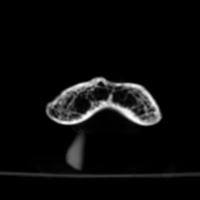
\includegraphics[width=1\textwidth]{../images/humerus/humerus_template1.png}
        \caption{}
     \end{subfigure}
\begin{subfigure}[b]{0.155\linewidth}
        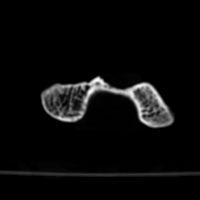
\includegraphics[width=1\textwidth]{../images/humerus/humerus_template2.png}
        \caption{}
     \end{subfigure}
\begin{subfigure}[b]{0.155\linewidth}
        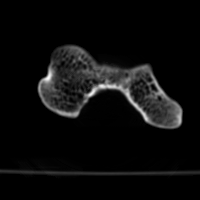
\includegraphics[width=1\textwidth]{../images/humerus/humerus_template3.png}
        \caption{}
     \end{subfigure}
\begin{subfigure}[b]{0.155\linewidth}
        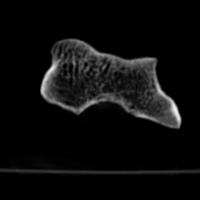
\includegraphics[width=1\textwidth]{../images/humerus/humerus_template4.png}
        \caption{}
     \end{subfigure}
\begin{subfigure}[b]{0.155\linewidth}
        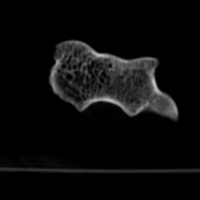
\includegraphics[width=1\textwidth]{../images/humerus/humerus_template5.png}
        \caption{}
     \end{subfigure}
\begin{subfigure}[b]{0.155\linewidth}
        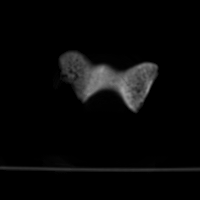
\includegraphics[width=1\textwidth]{../images/humerus/humerus_template6.png}
        \caption{}
     \end{subfigure}}\\
\begin{subfigure}[b]{0.235\linewidth}
        \fcolorbox{yellow}{yellow}{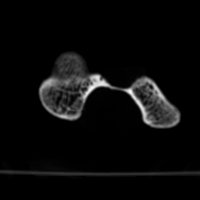
\includegraphics[width=\textwidth]{../images/humerus/global_local/groundTruth.png}}
        \caption{Test}
\end{subfigure}
\quad
    \begin{subfigure}[b]{0.23\linewidth}
        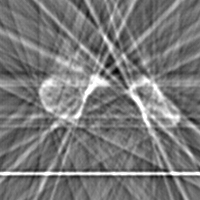
\includegraphics[width=\textwidth]{../images/humerus/fbp_humerus.png}
        \caption{FBP}
     \end{subfigure}
    \begin{subfigure}[b]{0.23\linewidth}
        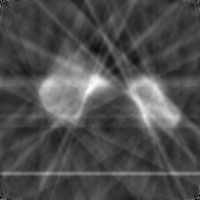
\includegraphics[width=\textwidth]{../images/humerus/global_local/reconNoPrior.png}
        \caption{CS}
    \end{subfigure}
    \begin{subfigure}[b]{0.23\linewidth}
        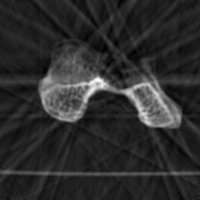
\includegraphics[width=\textwidth]{../images/humerus/global_local/global.png}
        \caption{This paper}
     \end{subfigure}
    \caption{\textit{Knowing more about the data helps.} Reconstructions of (g) a test slice  of size $(200,200)$ from the Humerus CT dataset~\cite{humerus} are performed using object-prior [(a)-(f)] and from measurements obtained from only 10 views. (h) Filtered backprojection (FBP) shows streaky sub-sampling artefacts (i) CS reduces the artefacts significantly while slightly blurring details (j) Prior information coupled with CS greatly improves the reconstruction.}
\label{fig:diff_methods}
\end{figure}

In addition, when some extra information about the object's structure is known~\cite{PICCS,cardiacPICCS,lubner2011,pirple,mota2017}, it is beneficial in further reducing the number of measurements.  These prior-based techniques use information from previously scanned data (`object-prior') of the same object or a similar one, and utilize it to reconstruct new volumes from very few sets of additional measurements. However, the above methods have the following two limitations: (1) the prior information may potentially overwhelm the essential details that appear in the test, (2) there is the key issue of choice of \textit{a} particular previously scanned object among the many previously acquired scans. A large part of this paper is dedicated to alleviating the former limitation, which is an important issue that has so far been overlooked in the literature on tomography. The latter limitation was relaxed in~\cite{liu2016,Xu2012} by building dictionary-based priors from multiple previously scanned objects. However, as reported in~\cite{my_dicta_paper}, dictionary priors are not as accurate and fast as global eigenspace priors.  Global eigenspace priors are better able to exploit the similarity of a test volume to object-prior, by assuming that the new test volume lies within the space spanned by the eigenvectors of the multiple representative previously scanned objects. Fig.~\ref{fig:diff_methods} shows the advantage of combining the global prior with CS.
\subsection{\textbf{Contributions}}
\label{sec:contributions}
In this work (Fig.~\ref{fig:prior_overview}), we focus on further reducing the number of measurements, with  particular emphasis on longitudinal studies. For example, we consider medical datasets which consist of multiple CT scans being taken during a radio-frequency ablation procedure~\cite{Dong2015}. The process consists of inserting a needle probe into a patient's body. When the needle reaches the tumor site, an electric current is passed to burn the tumor. Repeated CT scans of the patient need to be acquired in order to visualize the movement of the needle and to ensure that it is reaching the appropriate target. A few initial densely-sampled scans are used as object-prior to help the physician know the position of the needle. The later scans are used to reveal the exact changes during and after burning of the tumor (ablation).  In this context, we demonstrate the combined use of CS with the global prior, in two flavors: the vanilla (unselective) and selective global prior-based reconstruction. The choice of the number of measurement views and the type of reconstruction - unselective or selective, is driven by the goal of the procedure. 

\begin{figure}[h]
\centering
	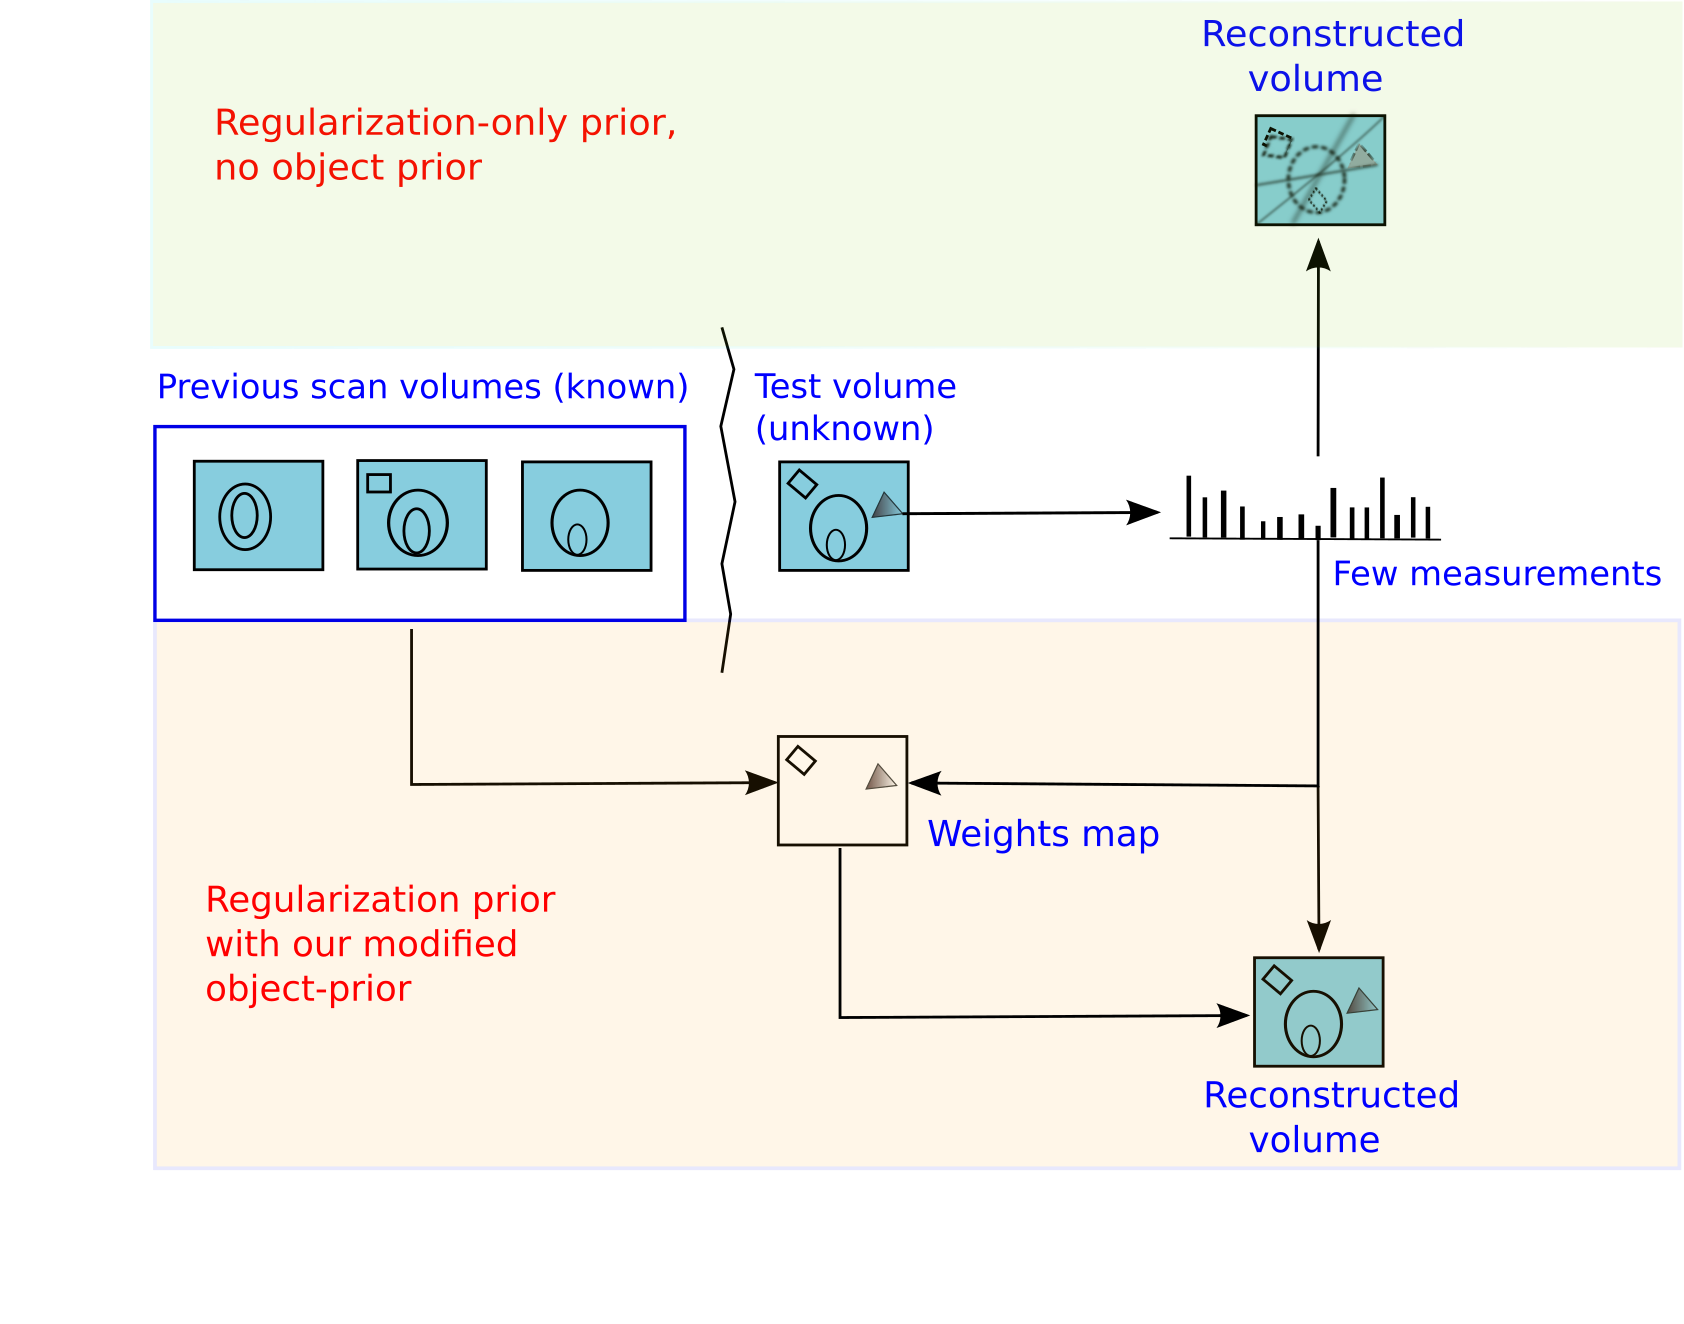
\includegraphics[width=0.5\textwidth]{../images/prior_cmb.png}
        \caption{Overview of our work. The choice of the number of measurement views and the type of reconstruction is driven by the goal in the application under consideration.  When our goal is relatively simple, such as tracking the location of new changes while simultaneously reducing sub-sampling artefacts, we propose (a) acquiring measurements from a small number of views (`few-view' imaging) and using unselective prior based reconstruction. When our goal becomes more ambitious, such as observing details of the new changes while simultaneously reducing sub-sampling artefacts, we propose (b) acquiring measurements from a slightly higher number of views (`moderate-view' imaging) and using selective prior-based reconstruction. In either case, the number of views is lower than what is conventionally used.}
 \label{fig:prior_overview}
\end{figure}

\begin{enumerate}
\item Initially, when our goal is to only track the location of the probe while simultaneously reducing sub-sampling artefacts, we advocate capturing measurements from a small number of views (`few-view' imaging) and using unselective prior based reconstruction. 
\item Later, when the probe is proximal to or touches the tumor, our goal is to observe details of tumor ablation while simultaneously reducing sub-sampling artefacts. In this case, we propose to capture measurements from a slightly higher number of views (`moderate-view' imaging) to acquire more information, and use a selective prior-based reconstruction. The selective technique moderates the effect of the prior in the reconstruction of new changes in the object being scanned.
\end{enumerate}
  
After the results of the above study are presented, the remainder of this paper discusses each of the above two approaches in detail. Specifically, we discuss how the global prior can impose an inflexible constant weight (and hence a bias) when reconstructing the data. If we want to observe details, this bias can be removed by moderating the control of the prior by imposing spatially varying weights to the prior. 

This paper is organized as follows: Section~\ref{sec:tmh} demonstrates the utility of both the unselective and selective methods on a longitudinal medical dataset. Section~\ref{sec:unselective_global_prior} describes the construction of the unselective global eigenspace prior. In addition, we recap the advantages of global prior over dictionary priors. Section~\ref{sec:selective_prior} describes how the unselective prior needs to be modified when accurate details of new changes are to be observed. A selective technique offers a solution. Results validated on both synthetic and real 3D biological datasets are shown. Finally, we conclude with key inferences that can be drawn from our work in Section~\ref{sec:conclusions}.


%--------------------------------THM section-------------------------

\section{Application: Reconstruction for CT-guided radio-ablation study}
\label{sec:tmh}
Before diving into the details of the unselective and the selective global prior methods, we first show how both the techniques can be applied to our advantage in a real-life medical longitudinal study. Longitudinal studies, in general, refer to the process of taking multiple CT scans of an object over specific intervals of time in order to study the evolution of the changes taking place in its interior. Here, our data~\footnote{Source: Tata Memorial Centre~\cite{tmh}, Parel, Mumbai.  This is the national comprehensive centre for the prevention, treatment, education and research in cancer, and is recognized as one of the leading cancer centres in India.} consists of CT scans from one such medical procedure. This involves successive scans of the liver taken during a radio-frequency ablation procedure described in the previous section. In such a procedure, the physician inserts a thin needle-like probe into the organ~\cite{rfa}. Once the needle hits the tumor, a high-frequency current is passed through the tip of the probe and this burns the malignant tumor. Throughout this process, multiple CT scans help the physician to track the position of the needle and check the changes within. In this context, we classify the goal of any of our reconstruction techniques into two categories: 

%--------------------------Results on TMH data--------------------------
%------------------RFA 2 data
\begin{figure}[h!]
    \begin{subfigure}[b]{0.24\linewidth}
        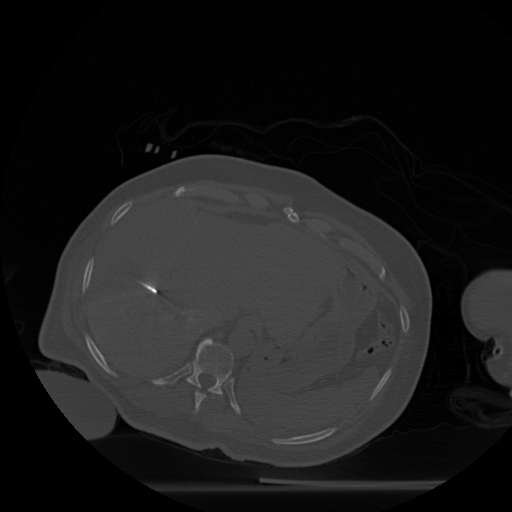
\includegraphics[width=\textwidth]{../images/tmh/RFA2/template1.png}
%\captionsetup{labelformat=empty}       
 \caption{slice 1}
    \end{subfigure}
    \begin{subfigure}[b]{0.24\linewidth}
        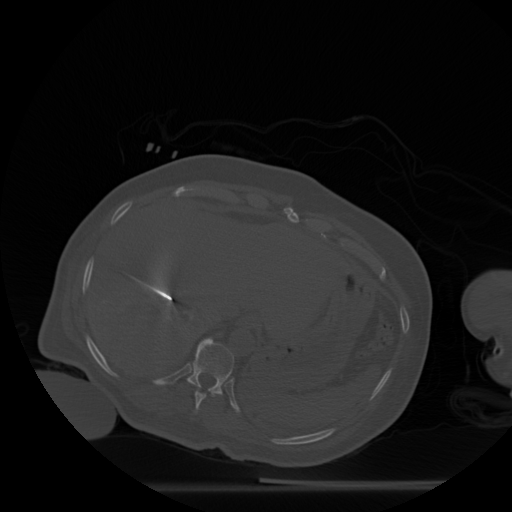
\includegraphics[width=\textwidth]{../images/tmh/RFA2/template2.png}
%\captionsetup{labelformat=empty}       
 \caption{slice 2}
    \end{subfigure}
     \begin{subfigure}[b]{0.24\linewidth}
        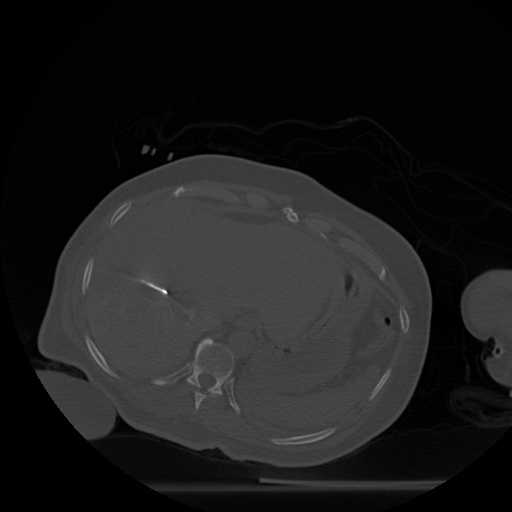
\includegraphics[width=\textwidth]{../images/tmh/RFA2/template3.png}
%\captionsetup{labelformat=empty}       
 \caption{slice 3}
    \end{subfigure}
       \begin{subfigure}[b]{0.24\linewidth}
        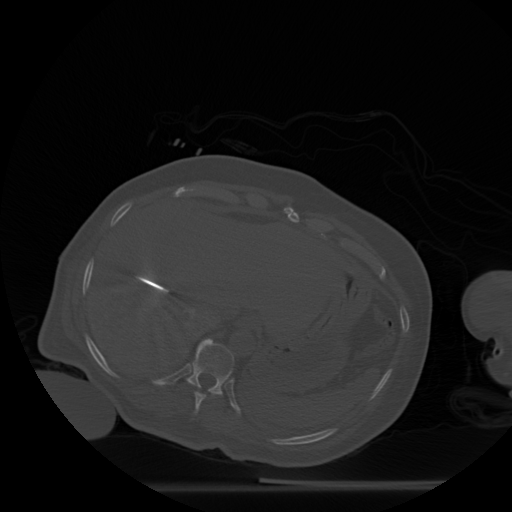
\includegraphics[width=\textwidth]{../images/tmh/RFA2/template4.png}
%\captionsetup{labelformat=empty}       
 \caption{slice 4}
    \end{subfigure}
       \begin{subfigure}[b]{0.24\linewidth}
        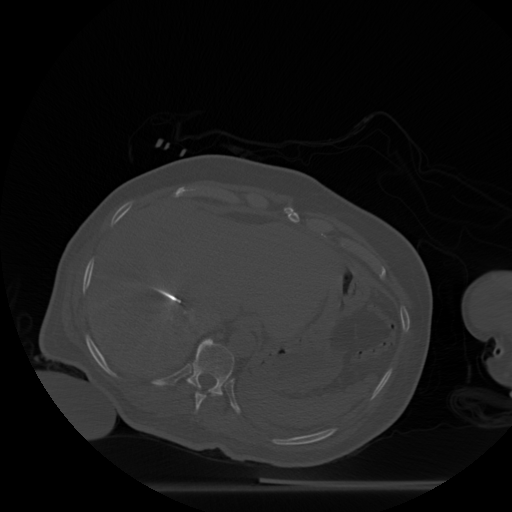
\includegraphics[width=\textwidth]{../images/tmh/RFA2/template5.png}
%\captionsetup{labelformat=empty}       
 \caption{slice 5}
    \end{subfigure}
              \begin{subfigure}[b]{0.24\linewidth}
        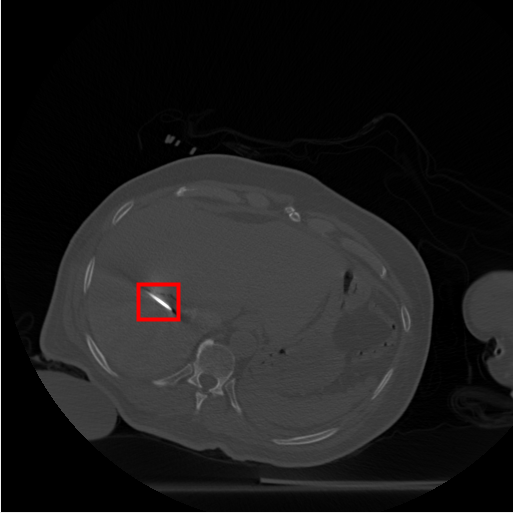
\includegraphics[width=\textwidth]{../images/tmh/RFA2/template6_color.png}
%\captionsetup{labelformat=empty}       
 \caption{slice 6}
    \end{subfigure}
       \begin{subfigure}[b]{0.24\linewidth}
        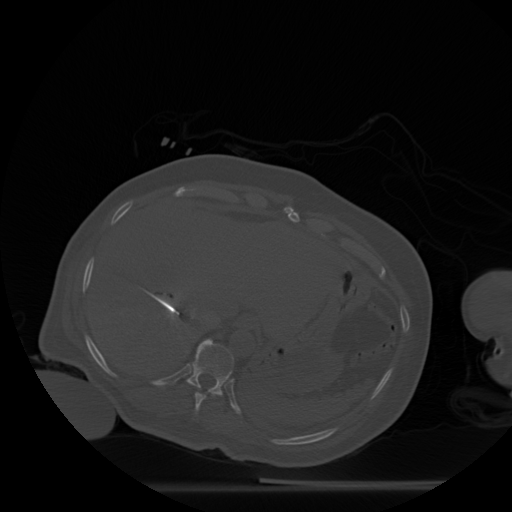
\includegraphics[width=\textwidth]{../images/tmh/RFA2/template7.png}
%\captionsetup{labelformat=empty}       
 \caption{slice 7}
    \end{subfigure}
       \begin{subfigure}[b]{0.24\linewidth}
        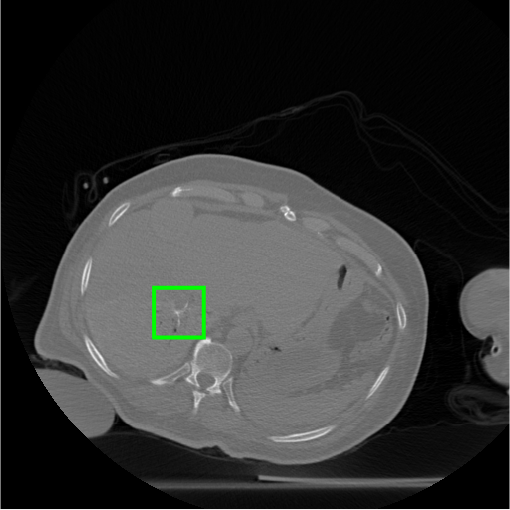
\includegraphics[width=\textwidth]{../images/tmh/RFA2/colorTestIm_ablation.png}
%\captionsetup{labelformat=empty}       
 \caption{slice 8}
    \end{subfigure}     
     \caption{Radio-frequency ablation dataset: One of the slices (512 x 512) from each of the 8 scan volumes of a longitudinal study dataset of the liver. Note that in volumes (a) through (g), the needle (shown in red in (f)) approaches the target tumor. (h) the organ after the ablation: this slice is displayed on a separate intensity scale to enable proper viewing of the region marked in green that shows the after-effects of ablating the tumor.} 
\label{fig:RFA2_test_object-prior}
\end{figure}

%--------------------RFA 2 few views
\begin{figure}[!h]
\centering
\subcaptionbox{Test}{\fcolorbox{white}{green}{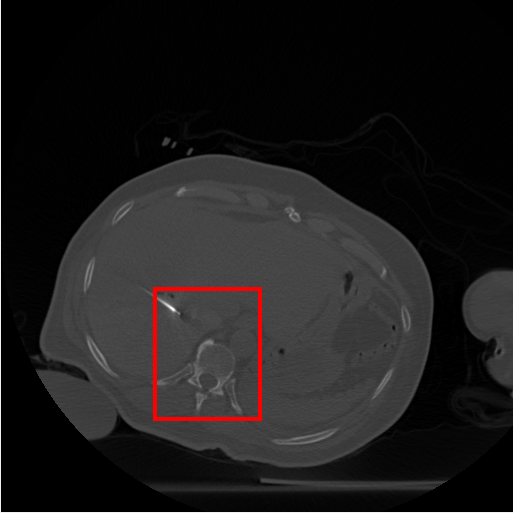
\includegraphics[width=0.23\columnwidth]{../images/tmh/RFA2/very_few_views/colorTestIm.png}}}\hfill
\subcaptionbox{Backprojection}{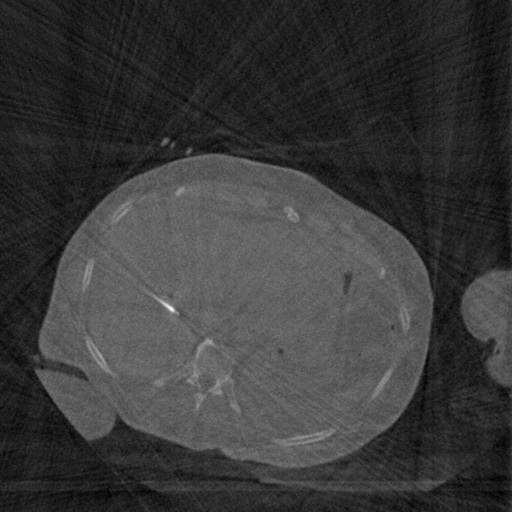
\includegraphics[width=0.24\columnwidth]{../images/tmh/RFA2/very_few_views/fbp.png}}\hfill
\subcaptionbox{CS}{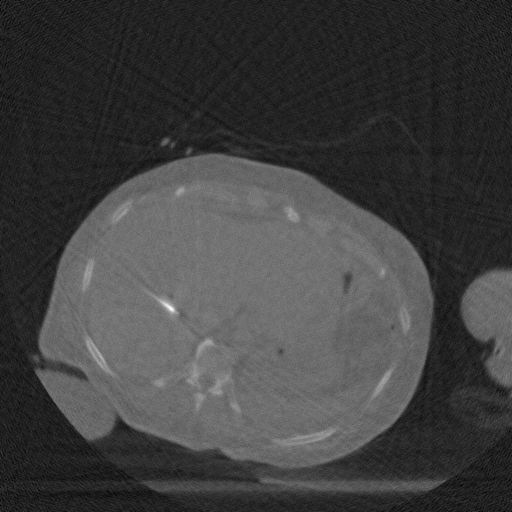
\includegraphics[width=0.24\columnwidth]{../images/tmh/RFA2/very_few_views/cs.png}}\hfill
\subcaptionbox{Proposed\\ method: unselective prior}{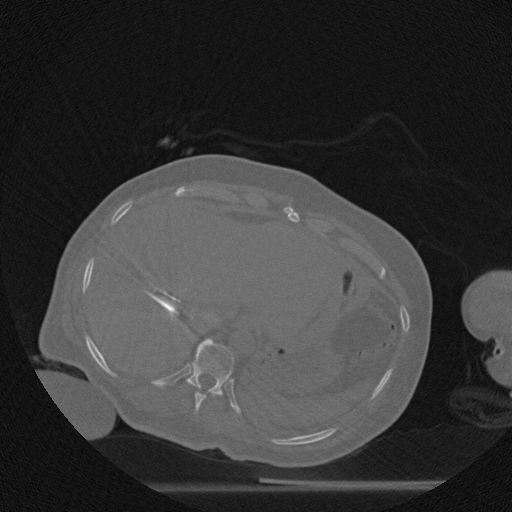
\includegraphics[width=0.24\columnwidth]{../images/tmh/RFA2/very_few_views/plain_pca.png}}
\caption[Representative results-1]{\textbf{Goal: Track new changes.}\small{ Reconstruction of slice 7 (`test') of Fig.~\ref{fig:RFA2_test_object-prior} from only 90 views, using (b) Filtered backprojection and no prior resulting in streaks, SSIM $= 0.48$ (c) CS and no prior resulting in blurred bone structures, SSIM $=0.35$ and (d) unselective global prior (slices 1-6 of Fig.~\ref{fig:RFA2_test_object-prior} are used as object-prior) resulting in clear bone structures with less streaks, SSIM $=0.55$. The region enclosed in red rectangle is our RoI as it contains both the new position of the needle and some background. All SSIM values are computed for this RoI.}}
\label{fig:RFA2_very_few_views}
\end{figure}

%-------RFA2 moderate views

\begin{figure}[!h]
\centering
\subcaptionbox{Test}{\fcolorbox{white}{blue}{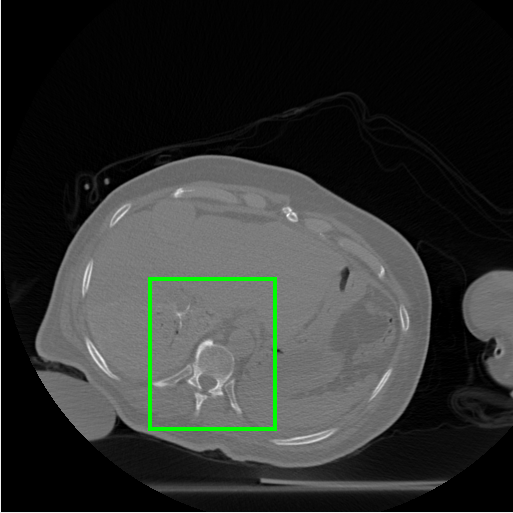
\includegraphics[width=0.23\columnwidth]{../images/tmh/RFA2/few_views/colorTestIm.png}}}\hfill
\subcaptionbox{Backprojection}{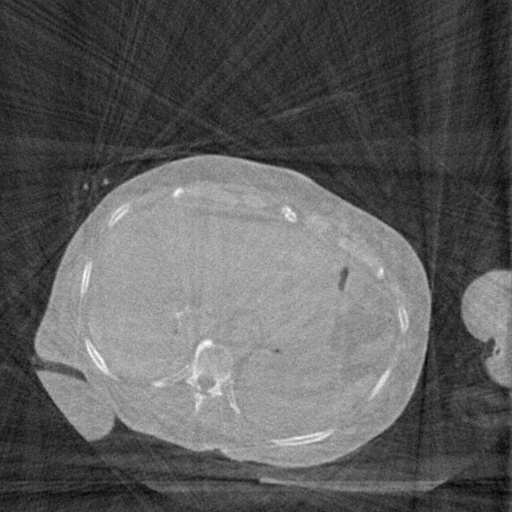
\includegraphics[width=0.24\columnwidth]{../images/tmh/RFA2/few_views/fbp.png}}\hfill
\subcaptionbox{CS}{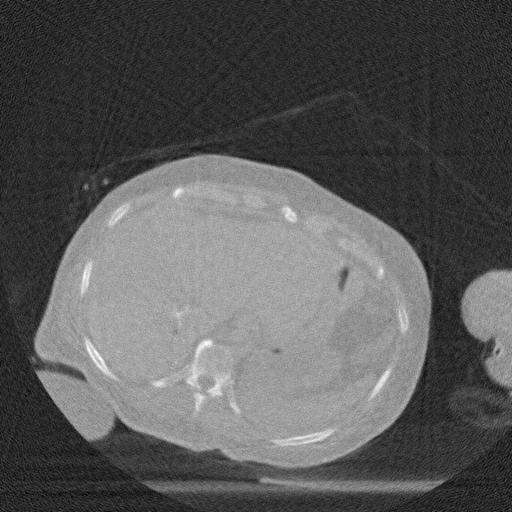
\includegraphics[width=0.24\columnwidth]{../images/tmh/RFA2/few_views/cs_dct.png}}\hfill
\subcaptionbox{Proposed\\ method: unselective\\ prior}{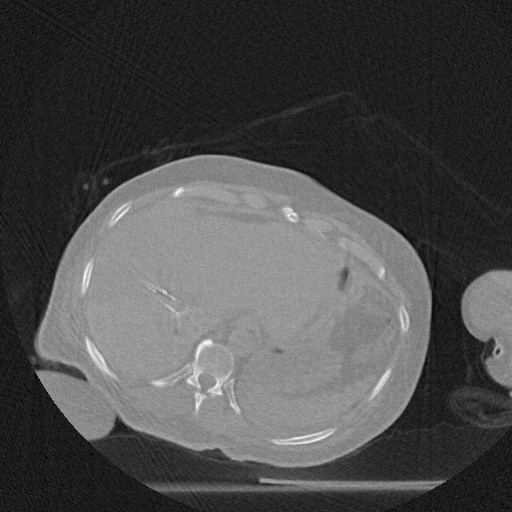
\includegraphics[width=0.24\columnwidth]{../images/tmh/RFA2/few_views/plain_pca.png}}
\subcaptionbox{Proposed\\ method: selective prior}{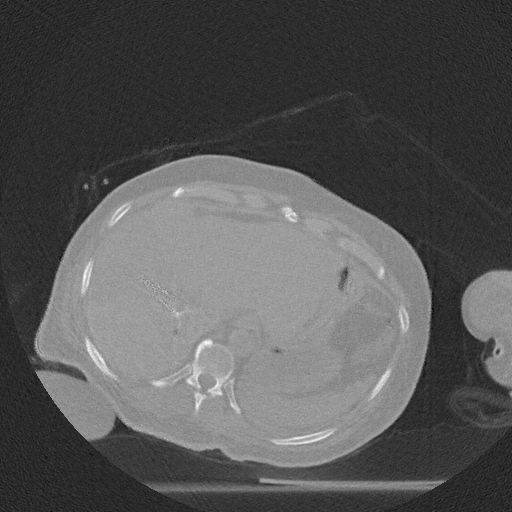
\includegraphics[width=0.24\columnwidth]{../images/tmh/RFA2/few_views/weighted_pca_all_methods_kk_0_01.png}}
\subcaptionbox{Weights map}{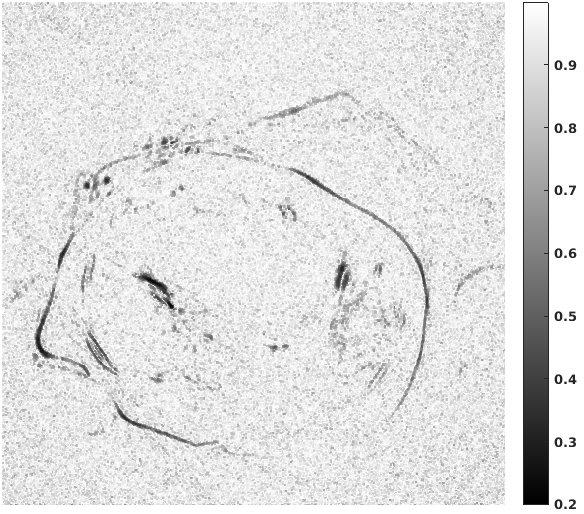
\includegraphics[width=0.275\columnwidth]{../images/tmh/RFA2/few_views/weights_colormap.png}}
\caption[Representative results-2]{\textbf{Goal: Observe details of new changes.} Reconstruction of slice 8 of Fig.~\ref{fig:RFA2_test_object-prior} from 120 views, using (b) FBP with SSIM $= 0.50$ (c) CS with SSIM $=0.46$ and (d) unselective global prior, with SSIM $=0.51$ (\emph{notice dominance of the prior: a prominent residual shadow of the needle which was present in the object-prior, but not present in the test image}), and (e) selective prior with SSIM $=0.56$ (\emph{notice that the dominance of the prior is significantly controlled}). The region enclosed in green rectangle is our Region of Interest (RoI) as it contains both the new position of the needle and some background. The SSIM is computed in this RoI. (f) shows the computed weights map (defined later in the paper) used for reconstruction. Darker intensities indicate lower weights to prior as these are the regions of new changes.}
\label{fig:RFA2_few_views}
\end{figure}

\begin{enumerate}
\item To track the position of the needle in a relatively well reconstructed background.
\item To accurately observe the new changes amidst a relatively well reconstructed background after the needle touches the tumor.
\end{enumerate} 

The needle has a very high attenuation coefficient when compared to that of the organs. Hence, the needle can be tracked by acquiring measurements from a very small number of views. We use the unselective global prior reconstruction here to reduce the artefacts due to sub-sampling. The unselective method is fast and sufficient to track the position of the needle.  Once the needle reaches the site of the tumor, we propose changing the imaging protocol to acquire measurements from a moderate number of views. This will enable us to get more information about the new changes. In addition, we then deploy the selective prior method in order to locate the regions of new changes and penalize any dominance of the prior in these regions.  Regardless of the imaging protocol we use (`few' or `moderate'), the number of views is smaller (atleast one-fifth) than the conventional number of views used in a standard hospital setting.

The dataset from this longitudinal medical study consists of 8 scans taken during the ablation procedure. We demonstrate our method for 2D reconstruction by choosing a single slice from each of the 8 volumes as our dataset. Note that all these 8 slices are located at the \emph{same} index~\footnote{The notion of~\textit{same index} (slice number corresponding to the same depth) makes sense in the context, because in such problems, the different scans are aligned with each other.} within each of the respective volumes. Fig.~\ref{fig:RFA2_test_object-prior} shows the chosen set of 2D slices (each of size $512 \times 512$) from the different volumes. Observe that the needle is seen in all of the first 7 slices  and the effect of ablation is seen in the 8th slice. \\

\textbf{Tracking the needle:} We first choose slices 1-6 as our object-prior, and reconstruct slice 7 with the specific goal of tracking the needle and simultaneously reduce artefacts. Fig.~\ref{fig:RFA2_very_few_views} shows the reconstruction of slice 7 from its measurements from only 90 views. The reconstructions are quantitatively compared using the Structural Similarity Index Metric (SSIM).\\ 

\textbf{Observing details of the ablation:} Next, we choose slices 1-7 as our object-prior and reconstruct slice 8 from 120 views i.e. a somewhat higher number of views this time. Fig.~\ref{fig:RFA2_few_views} shows the reconstructions of slice 8 by different methods. We see that the selective prior reconstruction brings in the advantage of the prior without it adversely affecting the new regions.

%---------------------------------Unselective section---------------------
\section{Methods}
\label{sec:methods}
Having presented the application, we first review the algorithm~\cite{my_dicta_paper} for a global (unselective) prior-based reconstruction in Sec.~\ref{sec:unselective_global_prior}. This is followed by details of our technique in Sec.~\ref{sec:selective_prior}. Our method estimates the location and magnitude of new changes, and eventually prevents the prior from adversely affecting the reconstruction of new regions in the test. This, we refer to as a \textit{selective} global prior-based reconstruction routine.
\subsection{\textbf{Summary of unselective global prior-based reconstruction}}
\label{sec:unselective_global_prior}

Principal Component Analysis (PCA) has been traditionally used to find the significant modes of (Gaussian corrupted) data. In this regard, it has been widely applied in the context of data compression. However, PCA can also be seen as a tool to provide an orthogonal basis to represent the space in which the test data could lie. This space is constructed from the available set of previously scanned objects which must cover a realistically representative range of structures. We first present the eigenspace-cum-CS prior-based reconstruction, which was shown~\cite{my_dicta_paper} to be better when compared to dictionary-based priors. %A preliminary version of this particular method was earlier presented in \cite{my_dicta_paper}. 

To begin with, when an object is scanned multiple times, a set of high quality reconstructions (i.e. reconstructions from a dense set of projection views) may be chosen as object-prior for the reconstruction of future scan volumes, which in turn, may be scanned using far fewer measurements. The eigenspace $E_{\text{high}}$ of the $L$ previously scanned objects $Q_1,Q_2,...,Q_L$ is pre-computed. Here, it is assumed that the test volume can be expressed as a sparse linear combination of the principal components (eigenvectors of the covariance matrix) obtained from a group of structurally similar volumes. Hence, the object-prior is represented by means of PCA. For the eigenspace to encompass a range of possible structures in the test slice, the object-prior must represent a wide structural range. Moreover, if these volumes are not aligned, then they must be first registered before computing the prior. The prior is built by computing the covariance matrix from the template set $\{Q_i\}_{i=1}^L$. \emph{The space spanned by the eigenvectors $\{\boldsymbol{V_k}\}_{k=1}^{L-1}$ (eigenspace) of the covariance matrix is the global prior and is assumed to contain any test slice that is similar, but not necessarily identical to the object-prior.}  We use all of the $L-1$ orthogonal eigenvectors as a basis to represent the unknown test volume. Let $\boldsymbol{x} = \boldsymbol{\Upsilon\theta}$ denote the reconstructed volume, $\boldsymbol{y} = \boldsymbol{\mathcal{R} x}$ its measured tomographic projections, $\boldsymbol{\mathcal{R}}$ the tomographic projection operator, $\boldsymbol{\theta}$ the sparse coefficients of $\boldsymbol{x}$, $\boldsymbol{\Upsilon}$ the basis in which $\boldsymbol{x}$ is assumed to be sparse, $\boldsymbol{\mu}$ the mean of the previously scanned objects, and $\boldsymbol{\alpha}$ the vector of eigen-coefficients of the test scan, of which $\alpha_k$ is the $k^{\textrm{th}}$ element. Then, once the eigenspace is pre-computed, the test is reconstructed by minimizing the following cost function:
\vspace{4mm}
 \begin{equation}
   \setlength{\belowdisplayskip}{0pt} \setlength{\belowdisplayshortskip}{0pt}
\setlength{\abovedisplayskip}{-2pt} \setlength{\abovedisplayshortskip}{-2pt}
J_1(\boldsymbol{\theta,\alpha}) = \lVert\boldsymbol{\mathcal{R} x}- \boldsymbol{y}\rVert_2^2  + \lambda_1\lVert\boldsymbol{\theta}\rVert_1+\lambda_2\lVert\boldsymbol{x} - (\boldsymbol{\mu} + \sum_{k}\boldsymbol{V_k}\alpha_k)\rVert_2^2.
\label{Eq:main_prior}
\end{equation}
Here, $\lambda_1$, $\lambda_2$ are tunable weights given to the sparsity and prior terms respectively. The unknowns $\boldsymbol{\theta}$ and $\boldsymbol{\alpha}$
are solved by alternately minimizing $J_{\boldsymbol{\alpha}}(\boldsymbol{\theta})$ using a fixed $\boldsymbol{\alpha}$, and $J_{\boldsymbol\theta}(\boldsymbol{\alpha})$ using the resultant $\boldsymbol{\theta}$, where 
\begin{align}
J_{\boldsymbol{\alpha}}(\boldsymbol{\theta}) &\triangleq \lVert\boldsymbol{\mathcal{R} x- y}\rVert_2^2  + \lambda_1\lVert\boldsymbol{\theta}\rVert_1+\lambda_2\lVert\boldsymbol{x} - (\boldsymbol{\mu + V\alpha})\rVert_2^2, \\
J_{\boldsymbol\theta}(\boldsymbol{\alpha}) &\triangleq \lVert\boldsymbol{\Upsilon\theta} - (\boldsymbol{\mu + V\alpha})\rVert_2^2.
\end{align}
Note that $\boldsymbol{\theta}$ is solved for using the basis pursuit CS solver~\cite{l1ls}. Solving for $\boldsymbol{\alpha}$ leads to the closed form update:
\begin{equation}
\boldsymbol{\boldsymbol{\alpha}} = \boldsymbol{V}^T(\boldsymbol{\Upsilon \theta} -\boldsymbol{\mu}).
\end{equation}
 Optimal values of $\lambda_1, \lambda_2$ must be empirically chosen \textit{a priori}, based on the reconstructions of one of the template volumes (see also Sec.~\ref{sec:discussion}). The cost function described in Eq.~\ref{Eq:main_prior} is biconvex and the convergence of this optimization is guaranteed by the monotone convergence theorem.
 %---------------------------------------------------------
 \vspace{2mm}
\subsubsection{\textbf{Patch-based techniques}}
\label{sec:patch_based}
Next we present a comparison~\cite{my_dicta_paper} of the performance of the aforementioned PCA-based global prior with a prior that is based on construction of patch-wise dictionaries. In both cases, the reconstruction routine is based on typical CS techniques. The well-known K-SVD algorithm \cite{Aharon2006} was chosen for construction of patch-based dictionaries. For this, patches were extracted from each of the template volumes, from which an overcomplete dictionary was obtained. The basic aim of the K-SVD algorithm (or any overcomplete dictionary learning technique) is the compact linear representation of all these patches using the dictionary columns. Let $\boldsymbol{D}$ denote the dictionary learned, $N_p$ the total number of patches, and $\boldsymbol{H_i}$ the operator to extract the $i^{\textrm{th}}$ patch from the intermediate reconstructed slice/volume. Then, once $\boldsymbol{D}$ is computed in an earlier `training phase', each new test slice (or test volume) can be reconstructed by optimizing a cost function such as the one below:
\begin{multline}
J_2(\boldsymbol{\theta},\{\boldsymbol{\alpha_i}\}_{i=1}^{N_p}) = \lVert\boldsymbol{\mathcal{R}\Upsilon\theta}- \boldsymbol{y}\rVert_2^2  + \lambda_1\lVert\boldsymbol{\theta}\rVert_1 + \\ \frac{\lambda_2}{N_p}\sum_{i=1}^{N_p}\lVert \boldsymbol{H_i\Upsilon \theta}-\boldsymbol{D \alpha_i}\rVert_2^2 +\frac{\lambda_3}{ N_p}\sum_{i=1}^{N_p}\lVert\boldsymbol{\alpha_i}\rVert_1.
\label{Eq:main_patchBased}
\end{multline}
The reconstruction proceeds in an alternating manner, first by minimization of Eq.~\ref{Eq:primaryObj_patchBased} and then by minimization of Eq.~\ref{Eq:alpha_patchBased}. For both these, the solver in~\cite{l1ls} is used. For the former case, the cost function reduces to:
\begin{equation}
J_{\boldsymbol{\alpha}}(\boldsymbol{\theta}) = \lVert \boldsymbol{\mathcal{R} \Upsilon \theta}- \boldsymbol{y}\rVert_2^2  + \lambda_1\lVert\boldsymbol{\theta}\rVert_1 + \frac{\lambda_2}{N_p}\sum_{i=1}^{N_p}\rVert \boldsymbol{H_i \Upsilon \theta}-\boldsymbol{D \alpha_i}\rVert_2^2.
\label{Eq:primaryObj_patchBased}
\end{equation}
For each $i \in \{1,...,N_p\}$, the cost function reduces to:
\begin{equation}
J_{\boldsymbol{\theta}}(\boldsymbol{\alpha}_i) =  \lVert \boldsymbol{H_i \Upsilon \theta}-\boldsymbol{D\alpha_i}\rVert_2^2  + \frac{\lambda_3}{\lambda_2}\lVert\boldsymbol{\alpha_i}\rVert_1.
\label{Eq:alpha_patchBased}
\end{equation}
This summarizes the comparison with patch-based methods.
%----------------------------------------------------

\subsection{\textbf{Selective prior-based reconstruction}}
\label{sec:selective_prior}
\vspace{1mm}
\noindent \begin{boxedminipage}{0.5\textwidth} 
{\bf Schematic 1}: Motivation behind our algorithm. (The plus $\oplus$ and the
minus $\ominus$ operators denote set-union and set-difference respectively; precise details available
in Section~\ref{sec:thealgo}). 
%\vspace{0.2cm}

{\small
 Let \textcolor{blue}{prior $Q:=$ old regions ($O$)}\\
 Let \textcolor{blue}{test volume $\boldsymbol{x}:=$ old regions ($O$) $\oplus$ new regions ($N$)}\\
% \textbf{Steps:}     
    \begin{enumerate}
\item  Compute pilot reconstruction of $\boldsymbol{x}$. Let this be called $X$.\\ \textcolor{blue}{$X = O \oplus N \oplus Ar(O) \oplus Ar(N)$}, where \\ \textcolor{blue}{$Ar(O)$} denote the reconstruction artefacts that depend on the \textit{old} regions, the imaging geometry and the reconstruction method, and\\
 \textcolor{blue}{$Ar(N)$} denote the reconstruction artefacts that depend on the \textit{new} regions, imaging geometry and the reconstruction method.
\item  Note that \textcolor{blue}{$Q \ominus X = N \oplus Ar(O) \oplus Ar(N)$} gives the new regions, but along with lots of artefacts due to the imaging geometry (sparse views). To eliminate these unwanted artefacts, compute \textcolor{blue}{$Y = Q \oplus Ar(O)$} by simulating projections from $Q$ using the same imaging geometry used to scan $\boldsymbol{x}$, and then reconstructing a lower quality prior volume $Y$. 
    \item Note that \textcolor{blue}{$Y \ominus X = N \oplus Ar(N)$} contains the artefacts due to the new regions only. These are different for different reconstruction methods. To eliminate these method dependent artefacts, compute $Y$ and $X$ using different reconstruction methods. Let these be denoted by $Y^j$ and $X^j$ respectively.
    \item Compute
\vspace{-0.2cm}
           \textcolor{blue}{\begin{equation*}
            Y^1 \ominus X^1 = N \oplus Ar^1(N)
           \end{equation*}
\vspace{-0.5cm}
           \begin{equation*}
            Y^2 \ominus X^2 = N \oplus Ar^2(N)
           \end{equation*}}
\vspace{-0.4cm}
   \item  New regions are obtained by computing
\vspace{-0.2cm}
          \textcolor{blue}{\begin{equation*}
          (Y^1 \ominus X^1)\cap(Y^2 \ominus X^2)= N
          \end{equation*}}   
\vspace{-0.5cm}
    \item Finally, assign space-varying weights $\boldsymbol{W}$ based on step $5$.
    \end{enumerate}
\label{algo:newRegionDetection}
}
\end{boxedminipage}
%--------------------------------------------------
\\

Although the unselective global prior can be very useful in some circumstances, as was shown in Sec.~\ref{sec:tmh}, it poses a major limitation when we want accurate details of the new changes. While the unselective prior compensates very well for the possible artefacts due to sparse measurements, it dominates the regions with new changes masking the signal, as seen in Fig.~\ref{fig:RFA2_few_views}-d. Ideally, we will want to impose the prior only in the regions that are common between the test and object-prior.  Our selective prior based reconstruction overcomes this limitation by minimizing the following cost function:
\begin{equation}
%   \setlength{\belowdisplayskip}{0pt} \setlength{\belowdisplayshortskip}{0pt}
%\setlength{\abovedisplayskip}{-2pt} \setlength{\abovedisplayshortskip}{-2pt}
J_3(\boldsymbol{\theta},\boldsymbol{\alpha}) = \lVert\boldsymbol{\mathcal{R} x}-\boldsymbol{y}\rVert_2^2  + \lambda_1\lVert\boldsymbol{\theta}\rVert_1 +\lambda_2\lVert\boldsymbol{W}(\boldsymbol{x} - (\boldsymbol{\mu} + \sum_{k}\boldsymbol{V_k}\alpha_k))\rVert_2^2.
\label{eq:selective_prior}
\end{equation}
The key to our method is the discovery of a diagonal weights
 matrix $\boldsymbol{W}$, where $W_{ii}$ contains the (non-negative) weight assigned to the $i^{\textrm{th}}$ voxel of the prior. $\boldsymbol{W}$ is first constructed using some preliminary reconstruction methods (to be described in the following section), following which Eq.~\ref{eq:selective_prior} is used to obtain the final reconstruction. In regions of change in test data, we want lower weights for the prior when compared to regions that are similar to the prior.  
\vspace{2mm}
 \subsubsection{\textbf{Computation of weights matrix $\boldsymbol{W}$}}
Since the test volume (referred to as $\boldsymbol{x}$) is unknown to begin with, it is not possible to decipher the precise regions in $\boldsymbol{x}$ that are different from all the previously scanned objects (`object-prior'). We refer the reader to Schematic 1 that describes the evolution of the procedure used to detect the new regions in the unknown volume. We start with $X^{\text{fdk}}$, the initial backprojection reconstruction of the test volume using the Feldkamp-Davis-Kress (FDK) algorithm~\cite{FDK} in an attempt to discover the difference between the object-prior and the test volume. Let $\boldsymbol{V_{\text{high}}}$ be the eigenspace constructed from high-quality object-prior. However, the difference between $X^{\text{fdk}}$ and its projection onto the eigenspace $\boldsymbol{V_{\text{high}}}$ will detect the new regions along with  many false positives (false new regions). This is because, $X^{\text{fdk}}$ will contain many geometric-specific artefacts arising from sparse measurements (angle undersampling), which are absent in the high quality object-prior used to construct the eigenspace $\boldsymbol{V_{\text{high}}}$. To discover unwanted artefacts of the imaging geometry, in a counter-intuitive way, we generate \emph{low quality} reconstruction of the object-prior as described below.
\vspace{2mm}
\subsubsection{\textbf{Algorithm to compute weights-map $\boldsymbol{W}$}}
\label{sec:thealgo}
\begin{enumerate}

\item Perform a pilot reconstruction $X^{\text{fdk}}$ of the
  test volume $\boldsymbol{x}$ using FDK.

\item Compute low quality template volumes $Y^\text{fdk}$. 
In Schematic 1, for ease of exposition, we assumed a single
template. In the sequel, we assume $L$ previously scanned objects from which we build
an eigenspace. 
\vspace{-0.1cm}

  \begin{enumerate}
  \item Generate simulated measurements $\boldsymbol{y_{Q_i}}$ for every template $Q_i$, using the exact same projections views and imaging geometry with which the measurements $\boldsymbol{y}$ of the test volume $\boldsymbol{x}$ were acquired, and 
\item Perform $L$  preliminary FDK reconstructions of each of the $L$ object-prior from $\boldsymbol{y_{Q_i}}$.  Let this be denoted by $\{Y^{\text{fdk}}_i\}_{i=1}^L$.
  \end{enumerate}
\item Build eigenspace $\boldsymbol{V_{\text{low}}}$ from $\{Y^{\text{fdk}}_i\}_{i=1}^L$.  Let $P^{\text{fdk}}$ denote projection of $X^{\text{fdk}}$ onto $\boldsymbol{V_{\text{low}}}$. The difference between $P^{\text{fdk}}$ and $X^{\text{fdk}}$ will not contain false positives due to imaging geometry, but will have false positives due to artefacts that are specific to the reconstruction method used. To resolve this, perform steps $4$ and $5$.
%\vspace{-0.3cm}
\item Project with multiple methods.
%\vspace{-0.1cm}
  \begin{enumerate}
  \item Perform pilot reconstructions of the test using $M$ different
    reconstruction algorithms\footnote{CS~\cite{lasso}, Algebraic Reconstruction Technique (ART)~\cite{art},
     Simultaneous Algebraic Reconstruction Technique (SART)~\cite{sart} and  Simultaneous Iterative Reconstruction Technique (SIRT)~\cite{sirt}}. Let this set be denoted
    as $X \triangleq \{X^j\}_{j=1}^M$ where $j$ is an index for the
    reconstruction method, and $X^1 = X^{\text{fdk}}$. 

  \item From $\boldsymbol{y_{Q_i}}$, perform reconstructions of the template $Q_i$ using the $M$ different algorithms, for each of the $L$ previously scanned objects. Let this set be denoted by $Y \triangleq \{\{Y_{i}^j\}_{j=1}^M\}_{i=1}^L$ where $Y^{1}_i = Y^{\text{fdk}}_i$, $\forall i \in \{1,..,,L\}$.


  \item For each of the $M$ algorithms (indexed by $j$), build an eigenspace $\boldsymbol{V_\text{low}^j}$ from $\{Y_1^j,Y_2^j, \ldots, Y_{L}^j\}$. %($j=1..M$).

  \item Next, for each $j$,  project $X^j$  onto $\boldsymbol{V_\text{low}^j}$. Let this projection be denoted by $P^j$. To reiterate, this captures those parts of the test volume that lie in the subspace $\boldsymbol{V_\text{low}^j}$ (i.e. are similar to the template reconstructions). The rest, i.e. new changes and their reconstruction method-dependent-artefacts, are not captured by this projection and need to be eliminated.
  \end{enumerate}
%\vspace{-0.1cm}
\item To remove all reconstruction method dependent false positives, we compute $\min_{j}(|X^j(x,y,z) - P^j(x,y,z)|)$. (The intuition for using the `min' is provided in the paragraph immediately following step 6 of this procedure.)
\item Finally, the weight to prior for each voxel coordinate $(x,y,z)$ is given by
  \begin{equation} 
    \boldsymbol{W_v}(x,y,z) = (1+k(\min_{j}|X^j(x,y,z) - P^j(x,y,z)|))^{-1}.
  \end{equation}
\label{eq:weightsEq}
\end{enumerate}
\vspace{0.01mm}
Note that here $\boldsymbol{W_v}(x,y,z)$ represents the weight to the prior in the $(x,y,z)^{th}$ voxel. $\boldsymbol{W_v}(x,y,z)$ must be
low whenever the preliminary test reconstruction $X^j(x,y,z)$ is different from its projection $P^j(x,y,z)$ onto the prior eigenspace, for \emph{every} method $j \in \{1,...,M\}$. This is
because it is unlikely that \emph{every} algorithm would produce a significant artefact at a voxel, and hence we hypothesize that the large difference has arisen due to genuine structural changes. The parameter $k$ decides the sensitivity of the weights to the difference $|X^j(x,y,z) - P^j(x,y,z)|$ and hence it depends on the size of the new regions we want to detect.  
%It must be chosen empirically based on the reconstruction of one of the template
%volumes. 
We found that our final reconstruction results obtained by
solving Eq.~\ref{eq:selective_prior} were robust over a wide range of $k$ values, as discussed in Sec.~\ref{sec:discussion}.
%-------------------------------------------
\subsubsection{\textbf{Motivation for the use of multiple types of eigenspaces for the computation of weights}}



%-----------------------------potato data
\begin{figure}[!h]
    \begin{subfigure}[b]{0.24\linewidth}
        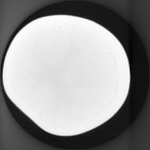
\includegraphics[width=\textwidth]{../images/potato/template_1.png}
\captionsetup{labelformat=empty}       
 \caption{}
    \end{subfigure}
    \begin{subfigure}[b]{0.24\linewidth}
        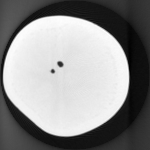
\includegraphics[width=\textwidth]{../images/potato/template_2.png}
\captionsetup{labelformat=empty}
        \caption{}
     \end{subfigure}
    \begin{subfigure}[b]{0.24\linewidth}
        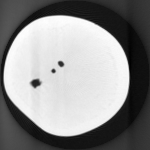
\includegraphics[width=\textwidth]{../images/potato/template_3.png}
\captionsetup{labelformat=empty}
        \caption{}
     \end{subfigure}
    \begin{subfigure}[b]{0.235\linewidth}
        \fcolorbox{yellow}{yellow}{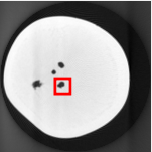
\includegraphics[width=\textwidth]{../images/potato/testIm_color.png}}
\captionsetup{labelformat=empty}
        \caption{}
\label{fig:potato_test}
     \end{subfigure}
      \caption{Potato dataset: One slice (slice-A) each from the previously scanned objects (the first three from left) and a slice from the test 
        volume (extreme right). Notice the appearance of the fourth
        hole in the test slice. }
\label{fig:object-prior_test_potato_A1}
\end{figure}

%-----------------------------potato 2D weights
\begin{figure}[!h]
    \begin{subfigure}[b]{0.24\linewidth}
        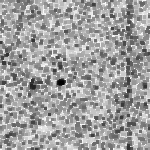
\includegraphics[width=\textwidth]{../images/potato/2D/weightsIm_fbp30.png}
        \caption{FBP}
    \end{subfigure}
    \begin{subfigure}[b]{0.24\linewidth}
        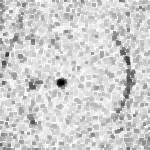
\includegraphics[width=\textwidth]{../images/potato/2D/weightsIm_cs_dct30.png}
        \caption{CS-DCT}
     \end{subfigure}
    \begin{subfigure}[b]{0.24\linewidth}
        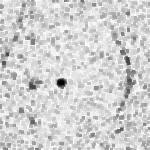
\includegraphics[width=\textwidth]{../images/potato/2D/weightsIm_cs_wavelet30.png}
        \caption{CS-Haar}
     \end{subfigure}
    \begin{subfigure}[b]{0.24\linewidth}
        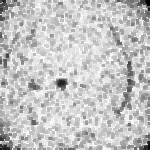
\includegraphics[width=\textwidth]{../images/potato/2D/weightsIm_art30.png}
        \caption{ART}
     \end{subfigure}
    \begin{subfigure}[b]{0.24\linewidth}
        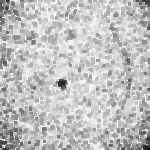
\includegraphics[width=\textwidth]{../images/potato/2D/weightsIm_sart30.png}
        \caption{SART}
     \end{subfigure}
    \begin{subfigure}[b]{0.24\linewidth}
        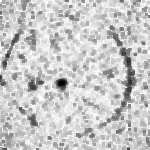
\includegraphics[width=\textwidth]{../images/potato/2D/weightsIm_sirt30.png}
        \caption{SIRT}
     \end{subfigure}
    \begin{subfigure}[b]{0.24\linewidth}
        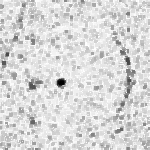
\includegraphics[width=\textwidth]{../images/potato/2D/weightsIm_all_methods30.png}
        \caption{combined}
     \end{subfigure}
      \caption{Weights-maps (corresponding to the difference between pilot reconstruction of the image in the last sub-figure of Fig.~\ref{fig:object-prior_test_potato_A1} and its projection onto the eigenspace $V_{low}$) constructed using different reconstruction methods, as specified in Eq.~\ref{eq:weightsEq}. The weights-maps are different because the reconstruction artefacts of the new structures in test image will be different for every reconstruction method used, as seen in Fig.~\ref{fig:reconstructions_diff_methods}. }
\label{fig:weights_map_2Dpotato}
\end{figure}
%-----------------------------potato 2D weights
\begin{figure}[!h]
    \begin{subfigure}[b]{0.24\linewidth}
        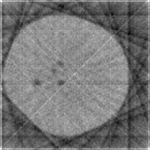
\includegraphics[width=\textwidth]{../images/potato/2D/fbp.png}
        \caption{FBP}
    \end{subfigure}
    \begin{subfigure}[b]{0.24\linewidth}
        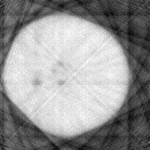
\includegraphics[width=\textwidth]{../images/potato/2D/cs_dct.png}
        \caption{CS-DCT}
     \end{subfigure}
    \begin{subfigure}[b]{0.24\linewidth}
        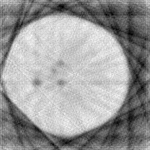
\includegraphics[width=\textwidth]{../images/potato/2D/cs_wavelet.png}
        \caption{CS-Haar}
     \end{subfigure}
    \begin{subfigure}[b]{0.24\linewidth}
        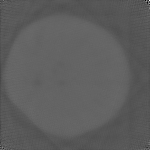
\includegraphics[width=\textwidth]{../images/potato/2D/art.png}
        \caption{ART}
     \end{subfigure}
    \begin{subfigure}[b]{0.24\linewidth}
        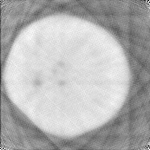
\includegraphics[width=\textwidth]{../images/potato/2D/sart.png}
        \caption{SART}
     \end{subfigure}
    \begin{subfigure}[b]{0.24\linewidth}
        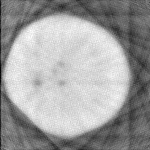
\includegraphics[width=\textwidth]{../images/potato/2D/sirt.png}
        \caption{SIRT}
     \end{subfigure}
    \begin{subfigure}[b]{0.24\linewidth}
        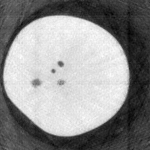
\includegraphics[width=\textwidth]{../images/potato/2D/weighted_pca_all_methods30.png}
        \caption{combined}
     \end{subfigure}
      \caption{(a)-(f):Different reconstructions of~\ref{fig:potato_test}. The magnitude and sharpness of the artefacts is different for each method. (g) Selective-prior method that combines weights-map information from all other methods.} 
\label{fig:reconstructions_diff_methods}
\end{figure}

The changes and new structures present in the test data will generate different artifacts for different reconstruction techniques. These artifacts would not be captured by reconstructions of the object-prior since the underlying new changes and structures may be absent in all of the previously scanned objects. We aim to let the weights be independent of the type of artifact. Hence, we use a combination of different reconstruction techniques to generate different types of eigenspaces and combine information from all of them to compute weights. To illustrate the benefit of this method, we first performed 2D reconstruction of a test slice from the potato dataset (please refer Sec.~\ref{Sec:potato} for details of the dataset) Fig.~\ref{fig:object-prior_test_potato_A1} shows the test and template slices. Fig.~\ref{fig:weights_map_2Dpotato}  shows the weights-maps generated using Eq.~\ref{eq:weightsEq} by various reconstruction methods. It can be seen that the weights are low in the region of the new change in test data. Because all the iterative methods are computationally expensive, we chose only FBP and CS-DCT for computing weights-maps for all 3D reconstructions.  


%----------------------------------------Results-----------------------
\section{Results}
\label{sec:results}

The proposed method has been validated on 2D and 3D synthetic and real tomographic data of biological and medical specimens. The results below demonstrate the advantage of the selective global prior method over the unselective method.


%\subsection{\textbf{Evaluation of selective prior-reconstruction in real 3D data}}

%-----------------------results of potato dataset


The proposed method has been validated on new\footnote {These and our code will be made available to the community.} scans of biological specimens in a longitudinal setting. These datasets in the form of \emph{raw cone-beam projection measurements} were acquired from a lab at the Australian National University (ANU). We emphasize that in most of the literature on tomographic reconstruction, the results are shown on reconstruction from projections \emph{simulated} from 3D volumes. This is because most CT scanners do not reveal the raw projections, and instead output only the full reconstructed volumes. Moreover, the process of conversion from the projections to the full volumes is proprietary. \emph{Departing from this, we demonstrate reconstruction results from raw projection data.} In all figures in this section, `unselective prior' refers to optimizing Eq.~\ref{eq:selective_prior} with $\boldsymbol{W}(x,y,z)=1$.
\begin{figure}[!h]
    \begin{subfigure}[b]{0.24\linewidth}
        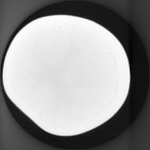
\includegraphics[width=\textwidth]{../images/potato/template_1.png}
\captionsetup{labelformat=empty}       
 \caption{}
    \end{subfigure}
    \begin{subfigure}[b]{0.24\linewidth}
        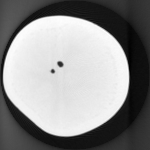
\includegraphics[width=\textwidth]{../images/potato/template_2.png}
\captionsetup{labelformat=empty}
        \caption{}
     \end{subfigure}
    \begin{subfigure}[b]{0.24\linewidth}
        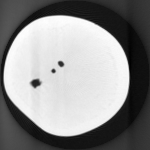
\includegraphics[width=\textwidth]{../images/potato/template_3.png}
\captionsetup{labelformat=empty}
        \caption{}
     \end{subfigure}
    \begin{subfigure}[b]{0.235\linewidth}
        \fcolorbox{blue}{blue}{\includegraphics[width=\textwidth]{../images/potato/testIm_color.png}}
\captionsetup{labelformat=empty}
        \caption{}
     \end{subfigure}
      \caption{Potato 3D dataset: One slice (slice-A) each from the previously scanned objects (the first three from left) and a slice from the test 
        volume (extreme right). Notice the appearance of the fourth
        hole in the test slice. }
\label{fig:object-prior_test_potato_A}
\end{figure}

%--------potato reconstruction--------------------------------------------------
\begin{figure}[!h]
\centering
\subcaptionbox{Test}{\fcolorbox{blue}{blue}{\includegraphics[width=0.185\columnwidth]{../images/potato/testIm_color.png}}}\hfill
\subcaptionbox{FDK, no prior}{\includegraphics[width=0.19\columnwidth]{../images/potato/fdkIm.png}}\hfill
\subcaptionbox{CS}{\includegraphics[width=0.19\columnwidth]{../images/potato/csIm.png}}\hfill
\subcaptionbox{\mbox{Unselective}\\prior}{\includegraphics[width=0.19\columnwidth]{../images/potato/plainPriorIm.png}}\hfill
\subcaptionbox{Selective\\ prior}{\includegraphics[width=0.19\columnwidth]{../images/potato/weightedPriorIm.png}}
\caption{Slice-A from 3D reconstruction of the potato with $5\%$ projection views--(b) has strong streak artefacts with unclear shadow of the potato, (c) largely blurred, (d) no new information detected (prior dominates) and (e) new information detected while simultaneously reducing streak artefacts. The reconstructed volumes can be viewed in~\cite{supp_paper}.}
\label{fig:potato_3D_results_A}
\end{figure}
%----------------------------------------------------------
%-----------------------results of potato dataset

\subsubsection{\textbf{Potato dataset}}
\label{Sec:potato}
The first (Potato) dataset consisted of four scans of the humble potato, chosen for its simplicity (Fig.~\ref{fig:object-prior_test_potato_A}). Measurements from each scan consisted of real cone-beam projections from 900 views, each of size $150\times150$. The corresponding size of the reconstructed volume is $150\times150\times100$. While the first scan was taken of the undistorted potato, subsequent scans were taken of the same specimen, each time after drilling a new hole halfway into the potato.  Projections were obtained using circular cone beam geometry. The specimen was kept in the same position throughout the acquisitions. In cases where such an alignment is not present, all the template volumes must be pre-aligned before computing the eigenspace. The test must be registered to the object-prior after its preliminary pilot reconstruction. %Further, this alignment can be refined following every update of the reconstructed test volume.
 The ground truth consists of FDK reconstructions from the full set of acquired measurements from 900 projection views. The test volume was reconstructed using measurements from 45 projection views, i.e. $5\%$ of the projection views from which ground truth was reconstructed.  The selected 3D
ground truth of template volumes, test volume, as well as the 3D reconstructions are shown in~\cite{supp_paper}. Fig.~\ref{fig:potato_3D_results_A} shows a slice from the reconstructed 3D volume. We observe that our method reconstructs new structures while simultaneously reducing streak artefacts.\\ %The new regions detected by different reconstruction methods are shown in Fig.~\ref{fig:weights_map_2Dpotato}. The lower intensities denote new regions which were assigned lower weights. This ensures that the new regions are reconstructed using projection measurements alone, avoiding erroneous influence of the prior.
%---------------------------------------
\begin{table}[!h]
\caption{SSIM of 3D reconstructed potato volumes from various methods. Each RoI spans 7 consecutive slices where the test is different from all of the previously scanned objects. In this dataset alone, the new changes are in a homogeneous background. Hence, the FDK performs the best when the RoI alone is considered. However, it fails when the entire volume is considered due to the prominent streaky artefacts.}
\begin{tabular}{|l|c|c|c|c|c|}
\hline
                   & \textbf{\begin{tabular}[c]{@{}c@{}}ground\\truth\end{tabular}} & \textbf{FDK} & \textbf{CS} & \textbf{\begin{tabular}[c]{@{}c@{}}Unselective\\prior + CS\end{tabular}} & \textbf{\begin{tabular}[c]{@{}c@{}}Selective\\prior + CS\end{tabular}} \\ \hline
\textbf{red RoI}   & 1 (ideal)                     & \textcolor{red}{0.939}        & 0.850       & 0.712                                                               & 0.852                                                            \\ \hline
\textbf{full volume} & 1 (ideal)                     & 0.744        & 0.817       & 0.856                                                               & \textcolor{red}{0.857}                                                                  \\ \hline
\end{tabular}
\label{table:potato_ssim}
\end{table}
%-------------------------------------------------
\subsubsection{\textbf{Okra dataset}}
\label{Sec:okra}
In order to test on data with intricate structures, a second (Okra) dataset consisting of five scans of an okra specimen was acquired (Fig.~\ref{fig:object-prior_test_okra}). The measurements consisted of real cone-beam projections from 450 views, each of size $336\times156$. The corresponding size of the reconstructed volume is $338\times338\times123$. Prior to the first scan, two holes were drilled on the surface of the specimen. This was followed by four scans, each after introducing one new cut. The ground truth consists of FDK reconstructed volumes from the the full set of 450 view projections. The test volume was reconstructed from a partial set of 45 projections, i.e. $10\%$ of the projection views from which ground truth was reconstructed. The selected 3D ground truth of template volumes, the test volume as well as the 3D reconstructions can be seen in~\cite{supp_paper}. One of the slices of the reconstructed volumes is shown in Fig.~\ref{fig:okra_3D_results}. The red and green 3D RoI in the video and images show the regions where new changes are present. Based on the potato and the okra experiments, we see that our method is able to \emph{discover both} the presence of a new structure, as well as the absence of a structure.

%--------------------------------okra data-------------------------------
\begin{figure}[!h]
    \begin{subfigure}[b]{0.18\linewidth}
        \includegraphics[width=\textwidth]{../images/okra/templateCropped_1.png}
\captionsetup{labelformat=empty}       
 \caption{}
    \end{subfigure}
    \begin{subfigure}[b]{0.18\linewidth}
        \includegraphics[width=\textwidth]{../images/okra/templateCropped_2.png}
\captionsetup{labelformat=empty}
        \caption{}
     \end{subfigure}
    \begin{subfigure}[b]{0.18\linewidth}
        \includegraphics[width=\textwidth]{../images/okra/templateCropped_3.png}
\captionsetup{labelformat=empty}
        \caption{}
     \end{subfigure}
    \begin{subfigure}[b]{0.18\linewidth}
        \includegraphics[width=\textwidth]{../images/okra/templateCropped_4.png}
\captionsetup{labelformat=empty}
        \caption{}
     \end{subfigure}
    \begin{subfigure}[b]{0.176\linewidth}
        \fcolorbox{yellow}{yellow}{\includegraphics[width=\textwidth]{../images/okra/testCropped.png}}
\captionsetup{labelformat=empty}
        \caption{}
     \end{subfigure}
     \caption{Okra 3D dataset: One slice each from the previously scanned objects (the
       first four from the left), and one from the test volume
       (extreme right). In the regions marked in red and green, while
       all slices have deformities, the test
       has none.}
\label{fig:object-prior_test_okra}
\end{figure}
%----------------------------------------------------

\begin{figure}[!h]
\centering
\subcaptionbox{Test}{\fcolorbox{yellow}{yellow}{\includegraphics[width=0.185\columnwidth]{../images/okra/testCropped.png}}}\hfill
\subcaptionbox{FDK, no prior}{\includegraphics[width=0.19\columnwidth]{../images/okra/fdk_cropped.png}}\hfill
\subcaptionbox{CS}{\includegraphics[width=0.19\columnwidth]{../images/okra/cs_cropped.png}}\hfill
\subcaptionbox{\mbox{Unselective}\\prior}{\includegraphics[width=0.19\columnwidth]{../images/okra/pca_cropped.png}}\hfill
\subcaptionbox{Selective\\ prior}{\includegraphics[width=0.19\columnwidth]{../images/okra/prior_weighted_cropped.png}}
\caption{3D reconstruction of the okra from $10\%$ projection
  views (b) has strong streak artefacts, (c) blurred, (d) no new
  information detected (prior dominates -- the deformity from the prior
  shows up as a false positive) and (e) new information detected (no deformities
  corresponding to red and green regions) while simultaneously
  reducing streak artefacts. The reconstructed volumes can be viewed in ~\cite{supp_paper}.}
\label{fig:okra_3D_results}
\end{figure}

%--------------------------------------zoomed okra

\begin{figure}[!h]
\centering
\subcaptionbox{Test}{\includegraphics[width=0.19\columnwidth]{../images/okra/zoomed/input_cropped.png}}\hfill
\subcaptionbox{FDK, no prior}{\includegraphics[width=0.19\columnwidth]{../images/okra/zoomed/FDK_cropped.png}}\hfill
\subcaptionbox{CS}{\includegraphics[width=0.19\columnwidth]{../images/okra/zoomed/CS_cropped.png}}\hfill
\subcaptionbox{\mbox{Unselective}\\prior}{\includegraphics[width=0.19\columnwidth]{../images/okra/zoomed/pca_cropped.png}}\hfill
\subcaptionbox{Selective\\ prior}{\includegraphics[width=0.19\columnwidth]{../images/okra/zoomed/weighted_prior_cropped.png}}
\caption{Zoomed in portion corresponding to the red RoI of Fig.~\ref{fig:okra_3D_results} for various methods (b) has strong streak artefacts, (c) blurred, (d) no new  information detected (prior dominates -- the deformity from the prior
  shows up as a false positive) and (e) new information detected (no deformities
 ).}
\label{fig:okra_zoomed_3D_results}
\end{figure}

%---------------------------------------
\begin{table}[!h]
  \caption{SSIM of 3D RoI of reconstructed okra volumes from various methods. Each RoI spans 7 consecutive slices where the test is different from all of the previously scanned objects.}
\begin{tabular}{|l|c|c|c|c|c|}
\hline
                   &  \textbf{\begin{tabular}[c]{@{}c@{}}Ground\\truth\end{tabular}} & \textbf{FDK} & \textbf{CS} & \textbf{\begin{tabular}[c]{@{}c@{}}Unselective\\prior + CS\end{tabular}} & \textbf{\begin{tabular}[c]{@{}c@{}}Selective\\prior + CS\end{tabular}} \\ \hline
\textbf{red RoI}   & 1 (ideal)                     & 0.737        & 0.836       & 0.858                                                               & \textcolor{red}{0.883}                                                                  \\ \hline
\textbf{green RoI} & 1 (ideal)                     & 0.798        & \textcolor{red}{0.861}       & 0.800                                                               & \textcolor{red}{0.861}                                                                  \\ \hline
\end{tabular}
\label{table:okra_ssim}
\end{table}



%-------------------------sprouts data

\begin{figure}[!h]
    \begin{subfigure}[b]{0.3\linewidth}
        \includegraphics[width=\textwidth]{../images/sprouts/template_1.png}
\captionsetup{labelformat=empty}
        \caption{}
    \end{subfigure}
\quad
    \begin{subfigure}[b]{0.3\linewidth}
        \includegraphics[width=\textwidth]{../images/sprouts/template_2.png}
\captionsetup{labelformat=empty}
        \caption{}
     \end{subfigure}
\quad
    \begin{subfigure}[b]{0.3\linewidth}
        \includegraphics[width=\textwidth]{../images/sprouts/template_3.png}
\captionsetup{labelformat=empty}
        \caption{}
     \end{subfigure}\\
    \begin{subfigure}[b]{0.3\linewidth}
        \includegraphics[width=\textwidth]{../images/sprouts/template_4.png}
\captionsetup{labelformat=empty}
        \caption{}
     \end{subfigure}
\quad
    \begin{subfigure}[b]{0.3\linewidth}
        \includegraphics[width=\textwidth]{../images/sprouts/template_5.png}
\captionsetup{labelformat=empty}
        \caption{}
     \end{subfigure}
\quad
    \begin{subfigure}[b]{0.29\linewidth}
        \fcolorbox{green}{green}{\includegraphics[width=\textwidth]{../images/sprouts/testIm_red.png}}
\captionsetup{labelformat=empty}
        \caption{}
     \end{subfigure}
      \caption{Sprouts 3D dataset: One slice each from the previously scanned objects (the first five from left) and a slice from the test (extreme
        right).}
\label{fig:object-prior_test_sprouts}
\addtolength{\textfloatsep}{-0.8cm}
\end{figure}
\subsubsection{\textbf{Sprouts dataset}}
\label{Sec:sprouts}
The third dataset consists of six scans of an in vivo
sprout specimen imaged at its various stages of growth
(Fig.~\ref{fig:object-prior_test_sprouts}). Projections were generated from the given volume of size $130\times130\times130$. In contrast to the scientific
experiment performed for the case of the okra and the potato where we
introduced man-made defects, the changes here are purely the work of
nature. %-----------------------------sprouts 3D results
\begin{figure}[!h]
    \begin{subfigure}[b]{0.29\linewidth}
        \fcolorbox{green}{green}{\includegraphics[width=\textwidth]{../images/sprouts/testIm_red.png}}
%\captionsetup{labelformat=empty}
        \caption{Test}
     \end{subfigure}
\quad
    \begin{subfigure}[b]{0.3\linewidth}
        \includegraphics[width=\textwidth]{../images/sprouts/fdkIm.png}
%\captionsetup{labelformat=empty}
        \caption{FDK}
    \end{subfigure}
\quad
    \begin{subfigure}[b]{0.3\linewidth}
        \includegraphics[width=\textwidth]{../images/sprouts/csIm.png}
%\captionsetup{labelformat=empty}
        \caption{CS}
     \end{subfigure}\\
\quad
    \begin{subfigure}[b]{0.3\linewidth}
        \includegraphics[width=\textwidth]{../images/sprouts/plainPriorIm.png}
%\captionsetup{labelformat=empty}
        \caption{Unselective Prior}
     \end{subfigure}
\quad
    \begin{subfigure}[b]{0.3\linewidth}
        \includegraphics[width=\textwidth]{../images/sprouts/weightedPriorIm.png}
%\captionsetup{labelformat=empty}
        \caption{Selective prior}
     \end{subfigure}
     \caption{3D reconstruction of sprouts from $2.5\%$ projection views
   (b, c) have poor details (d) no new information detected (the
   prior dominates as can be seen in the blue and red regions) and
   (e) new information detected in the regions of interest. The reconstructed volumes can be viewed in ~\cite{supp_paper}.} 
\label{fig:sprouts_3D_results}
%\addtolength{\textfloatsep}{-0.8cm}
\end{figure}

%--------------------------------------zoomed sprouts

\begin{figure}[!h]
\centering
\subcaptionbox{Test}{\includegraphics[width=0.19\columnwidth]{../images/sprouts/zoomed/input_cropped.png}}\hfill
\subcaptionbox{FDK, no prior}{\includegraphics[width=0.19\columnwidth]{../images/sprouts/zoomed/FDK_cropped.png}}\hfill
\subcaptionbox{CS}{\includegraphics[width=0.19\columnwidth]{../images/sprouts/zoomed/CS_cropped.png}}\hfill
\subcaptionbox{\mbox{Unselective}\\prior}{\includegraphics[width=0.19\columnwidth]{../images/sprouts/zoomed/pca_cropped.png}}\hfill
\subcaptionbox{Selective\\ prior}{\includegraphics[width=0.19\columnwidth]{../images/sprouts/zoomed/weighted_prior_cropped.png}}
\caption{Zoomed-in portion $(16 \times 21)$ corresponding to the red RoI of Fig.~\ref{fig:sprouts_3D_results} for various methods (b) unclear, (c) unclear, (d) only two strong structures seen and (e) there is a hint of a third structure too (as seen in the test RoI).}
\label{fig:sprouts_zoomed_3D_results}
\end{figure}

%--------------------------------------------------------------
\begin{table}[]
\caption{SSIM of 3D RoI of reconstructed sprouts volumes from various methods. The RoI spans 7 consecutive slices where the test is different from all of the previously scanned objects.}
\begin{tabular}{|l|c|c|c|c|c|}
\hline
                   & \textbf{\begin{tabular}[c]{@{}c@{}}ground\\truth\end{tabular}} & \textbf{FDK} & \textbf{CS} & \textbf{\begin{tabular}[c]{@{}c@{}}Unselective\\prior + CS\end{tabular}} & \textbf{\begin{tabular}[c]{@{}c@{}}Selective\\prior + CS\end{tabular}} \\ \hline
\textbf{red RoI}   & 1 (ideal)                     & 0.852        & 0.843       & 0.834                                                               & \textcolor{red}{0.881}                                                                  \\ \hline
\end{tabular}
\label{table:sprouts_ssim}
\end{table}
The ground truth consists of FDK reconstructed volumes from a set of
1800 view projections. The test volume was reconstructed from partial
set of 45 projections, i.e. $2.5\%$ of the projection views from which
ground truth was reconstructed. The selected 3D ground truth of
template volumes, test volume, as well as the 3D reconstructions are
shown in~\cite{supp_paper}. One of the slices of the
reconstructed volumes and its zoomed-in RoI are shown in
Figs.~\ref{fig:sprouts_3D_results} and ~\ref{fig:sprouts_zoomed_3D_results} respectively. For the sake of exposition, the red region of interest (RoI) has been culled out from 7
consecutive slices in the 3D volume to indicate new structures; other
changes can be viewed in the video. Tables~\ref{table:potato_ssim},~\ref{table:okra_ssim} and \ref{table:sprouts_ssim} show the improvement in the Structure
Similarity Index (SSIM) of the reconstructed new regions as compared
to other methods. 

\subsection{\textbf{More results on CT-guided radio-frequency ablation data}}

%-------------------- RFA 2 new protocol
\begin{figure}[!h]
       \begin{subfigure}[b]{0.24\linewidth}
        \includegraphics[width=\textwidth]{../images/tmh/RFA2/template1.png}
\captionsetup{labelformat=empty}       
 \caption{image-1}
    \end{subfigure}
       \begin{subfigure}[b]{0.24\linewidth}
        \includegraphics[width=\textwidth]{../images/tmh/RFA2/new_protocol/result_image_1.png}
\captionsetup{labelformat=empty}       
 \caption{image-1 recon}
    \end{subfigure}
 \begin{subfigure}[b]{0.24\linewidth}
        \includegraphics[width=\textwidth]{../images/tmh/RFA2/template2.png}
\captionsetup{labelformat=empty}       
 \caption{image-2}
    \end{subfigure}
       \begin{subfigure}[b]{0.24\linewidth}
        \includegraphics[width=\textwidth]{../images/tmh/RFA2/new_protocol/result_image_2.png}
\captionsetup{labelformat=empty}       
 \caption{image-2 recon}
    \end{subfigure}
 \begin{subfigure}[b]{0.24\linewidth}
        \includegraphics[width=\textwidth]{../images/tmh/RFA2/template3.png}
\captionsetup{labelformat=empty}       
 \caption{image-3}
    \end{subfigure}
       \begin{subfigure}[b]{0.24\linewidth}
        \includegraphics[width=\textwidth]{../images/tmh/RFA2/new_protocol/result_image_3.png}
\captionsetup{labelformat=empty}       
 \caption{image-3 recon}
    \end{subfigure}
 \begin{subfigure}[b]{0.24\linewidth}
        \includegraphics[width=\textwidth]{../images/tmh/RFA2/template4.png}
\captionsetup{labelformat=empty}       
 \caption{image-4}
    \end{subfigure}
       \begin{subfigure}[b]{0.24\linewidth}
        \includegraphics[width=\textwidth]{../images/tmh/RFA2/new_protocol/result_image_4.png}
\captionsetup{labelformat=empty}       
 \caption{image-4 recon}
    \end{subfigure}
 \begin{subfigure}[b]{0.24\linewidth}
        \includegraphics[width=\textwidth]{../images/tmh/RFA2/template5.png}
\captionsetup{labelformat=empty}       
 \caption{image-5}
    \end{subfigure}
       \begin{subfigure}[b]{0.24\linewidth}
        \includegraphics[width=\textwidth]{../images/tmh/RFA2/new_protocol/result_image_5.png}
\captionsetup{labelformat=empty}       
 \caption{image-5 recon}
    \end{subfigure}
 \begin{subfigure}[b]{0.24\linewidth}
        \includegraphics[width=\textwidth]{../images/tmh/RFA2/template6.png}
\captionsetup{labelformat=empty}       
 \caption{image-6}
    \end{subfigure}
       \begin{subfigure}[b]{0.24\linewidth}
        \includegraphics[width=\textwidth]{../images/tmh/RFA2/new_protocol/result_image_6.png}
\captionsetup{labelformat=empty}       
 \caption{image-6 recon}
    \end{subfigure}
 \begin{subfigure}[b]{0.24\linewidth}
        \includegraphics[width=\textwidth]{../images/tmh/RFA2/template7.png}
\captionsetup{labelformat=empty}       
 \caption{image-7}
    \end{subfigure}
       \begin{subfigure}[b]{0.24\linewidth}
        \includegraphics[width=\textwidth]{../images/tmh/RFA2/new_protocol/result_image_7.png}
\captionsetup{labelformat=empty}       
 \caption{image-7 recon}
    \end{subfigure}
 \begin{subfigure}[b]{0.24\linewidth}
        \includegraphics[width=\textwidth]{../images/tmh/RFA2/testIm.png}
\captionsetup{labelformat=empty}       
 \caption{image-8}
    \end{subfigure}
       \begin{subfigure}[b]{0.24\linewidth}
        \includegraphics[width=\textwidth]{../images/tmh/RFA2/new_protocol/weighted_pca_all_methods_kk_0_01.png}
\captionsetup{labelformat=empty}       
 \caption{image-8 recon}
    \end{subfigure}
       \begin{subfigure}[b]{0.24\linewidth}
        \includegraphics[width=\textwidth]{../images/tmh/RFA2/new_protocol/weightsIm_all_methods_kk_0_01.png}
\captionsetup{labelformat=empty}       
 \caption{weights map}
    \end{subfigure}
       \caption{Reconstructions (referred as `recon') of all slices of  of Fig.~\ref{fig:RFA2_test_object-prior} using the suggested protocol in Table.~\ref{tab:realistic_imaging_protocol}. The last image is the weights map corresponding to the reconstruction of image-8. The new changes in the tumor site is picked up by the weights map. }
\label{fig:RFA2_new_protocol}
\end{figure}

Earlier in Sec.~\ref{sec:tmh}, we discussed that the imaging protocols fell under two categories depending on the final goal (tracking or observing details): very few-view imaging and moderate view imaging. \textbf{Ideally, we may prefer to gradually increase from few-view to moderate views as the probe gradually approaches the tumor site.} For the reconstruction of $n^{\textrm{th}}$ slice i.e. slice imaged at time $t=n$, the few-view reconstructions of the previously acquired slices can be used as object-prior. However, the first scan must always be taken with large number of views because it acts as a reference template to start with. Table.~\ref{tab:realistic_imaging_protocol} summarizes this protocol for the dataset of Fig~\ref{fig:RFA2_test_object-prior}, and Fig.~\ref{fig:RFA2_new_protocol} shows the reconstructions when this realistic protocol is used.

\begin{table}[!h]
  \caption{Suggested multi-step imaging protocol for the CT-guided radio-frequency ablation dataset of Fig~\ref{fig:RFA2_test_object-prior}. The number of views is gradually increased as the probe approaches the tumor site. Only the first scan is taken with large number of views to act as a reference template. The few-view reconstructions of a slice acts as the object-prior for the reconstruction of slice being imaged at next time instant.}
  \vspace{2mm}
\centering\small\setlength\tabcolsep{2pt}
\hspace*{-1cm}
\begin{tabular}{|c|c|c|c|}
\hline
\textbf{\begin{tabular}[c]{@{}c@{}}Slice being\\ imaged at\\ time t\end{tabular}} & \textbf{\begin{tabular}[c]{@{}c@{}}Probe distance from\\ tumor or \\ ablation stage\end{tabular}} & \textbf{\begin{tabular}[c]{@{}c@{}}Number of\\ imaging\\ views\end{tabular}} & \textbf{\begin{tabular}[c]{@{}c@{}}Reconstruction\\ protocol: type \\ of global prior\end{tabular}} \\ \hline
Slice t=1 & Very far from tumor & 360 & CS \\ \hline
Slice t=2 & Sufficiently far from tumor & 40 & Unselective \\ \hline
Slice t=3 & Far from tumor & 50 & Unselective \\ \hline
Slice t=4 & Near tumor & 60 & Unselective \\ \hline
Slice t=5 & Sufficiently near tumor & 70 & Unselective \\ \hline
Slice t=6 & Very near tumor & 80 & Unselective \\ \hline
Slice t=7 & Very near tumor & 90 & Unselective \\ \hline
Slice t=8 & During, after ablation & 120 & Selective \\ \hline
\end{tabular}\hspace*{-1cm}
\label{tab:realistic_imaging_protocol}
\end{table}

%--------------------------------------------------------------------------
\section{Discussion}
\label{sec:discussion}
The presented unselective prior-based algorithm is suited to applications where we wish to detect the location of new changes in an object over time, and the presented selective prior-based algorithm is suited to applications where we wish to observe the intricate details of those new changes. This distinction in the techniques used has not been studied earlier in literature~\cite{geyer2015,PICCS,Ali2018,Tan2017} to the best of our knowledge. Eventhough methods such as~\cite{Hakka2019} offer the flexibility of using multiple templates, the very important issue of these templates overwhelming the current reconstruction has been largely ignored. We have presented a principled method of tackling this particular issue via our weights map. We not only estimate the location of new changes, but also compute their intensities. This information is then used to modulate the strength of the prior during the reconstruction of the test. Our results consist of 3D reconstructions from real cone-beam projections of two datasets, and both 3D and 2D reconstructions from cone-beam and parallel beam projections respectively. In each case, we have compared our results with those from standard back-projection algorithms~\cite{Pan2009} (FDK in case of 3D and FBP incase of 2D), and Compressed Sensing~\cite{Donoho,introCS} based reconstructions. An in-depth analysis of each of the results is presented in Sec.~\ref{sec:results}. We now discuss the need for registration between object-prior and the test, and the effect of hyper-parameters on our reconstructions.

\subsection{Issue of misalignment between test and templates}
As with any global prior-based method, there is a need for the test volume to be registered with the object-prior. In all our longitudinal study experiments, the volumes were already aligned during imaging. However, if this were not the case, then the prior must be aligned to the test based on an initial pilot reconstruction of the test.

\subsection{Effect of hyper-parameters}
\label{subsec:k}
The parameters $\lambda_1$ and $\lambda_2$ must be chosen empirically or by cross-validation by treating one of the previously scanned objects as test. In our experiments, we had fixed $\lambda_1$ to be 1 and found that this value is nearly data-independent. The value of $\lambda_2$ largely depends on the amount of artefacts we aim to remove by using prior at the cost of their dominance in the new regions. This value was chosen to lie between $0-1$ for our datasets. Finally, the hyper-parameter $k$ defines the sensitivity of the weights map to the difference between the test image and the prior (projection of test onto the space of object-prior). When $k=0$, our method converges to the unselective prior method. As $k$ increases, the weights map starts capturing the new changes in the test, at the cost of detecting a few false positives i.e. false new changes. In other words, as the weights map becomes more sensitive to the difference between the test and object-prior, it becomes more noisy. In order to visualize the effect of the hyper-parameter $k$, we performed 2D reconstructions of okra dataset for different values of $k$. Fig.~\ref{fig:few_view_okra_2D_weights} shows the weights map obtained for each of the $k$ values. We estimate an approximate choice for the optimal value of $k$ by treating one of the object-prior as test and reconstructing it. We also note that although the weights map is heavily influenced by $k$, the final reconstructions are stable for large variations in $k$, as seen in Fig.~\ref{fig:reconstructions_as_k_varies}. Alternatively, in cases where one wishes to completely avoid the use of this hyper-parameter, one can construct a binary weights-map using a learning based method described in~\cite{supp_paper}.

%--------------effect of the value of $k$ on Okra dataset


\begin{figure}[h]
    \begin{subfigure}[b]{0.24\linewidth}
        \includegraphics[width=\textwidth]{../images/okra/2D_okra/weightsIm_10normalized.png}
        \caption{k=10}
     \end{subfigure}     
  \begin{subfigure}[b]{0.24\linewidth}
        \includegraphics[width=\textwidth]{../images/okra/2D_okra/weightsIm_50normalized.png}
        \caption{k=50}
     \end{subfigure} 
  \begin{subfigure}[b]{0.24\linewidth}
        \includegraphics[width=\textwidth]{../images/okra/2D_okra/weightsIm_90normalized.png}
        \caption{k=90}
     \end{subfigure}
  \begin{subfigure}[b]{0.24\linewidth}
        \includegraphics[width=\textwidth]{../images/okra/2D_okra/weightsIm_130normalized.png}
        \caption{k=130}
     \end{subfigure}
  \begin{subfigure}[b]{0.24\linewidth}
        \includegraphics[width=\textwidth]{../images/okra/2D_okra/weightsIm_170normalized.png}
        \caption{k=170}
     \end{subfigure}
  \begin{subfigure}[b]{0.24\linewidth}
        \includegraphics[width=\textwidth]{../images/okra/2D_okra/weightsIm_210normalized.png}
        \caption{k=210}
     \end{subfigure}
   \begin{subfigure}[b]{0.24\linewidth}
        \includegraphics[width=\textwidth]{../images/okra/2D_okra/weightsIm_250normalized.png}
        \caption{k=250}
     \end{subfigure}
   \begin{subfigure}[b]{0.24\linewidth}
        \includegraphics[width=\textwidth]{../images/okra/2D_okra/weightsIm_290normalized.png}
        \caption{k=290}
     \end{subfigure}
  \begin{subfigure}[b]{0.24\linewidth}
        \includegraphics[width=\textwidth]{../images/okra/2D_okra/weightsIm_330normalized.png}
        \caption{k=330}
     \end{subfigure}
   \begin{subfigure}[b]{0.24\linewidth}
        \includegraphics[width=\textwidth]{../images/okra/2D_okra/weightsIm_370normalized.png}
        \caption{k=370}
     \end{subfigure}
   \begin{subfigure}[b]{0.24\linewidth}
        \includegraphics[width=\textwidth]{../images/okra/2D_okra/weightsIm_410normalized.png}
        \caption{k=410}
     \end{subfigure}
   \begin{subfigure}[b]{0.24\linewidth}
        \includegraphics[width=1.15\textwidth]{../images/okra/2D_okra/weightsIm_450normalized_colorbar.png}
        \caption{k=450}
     \end{subfigure}
    \caption{Different weights-maps for okra reconstruction. Low intensity denotes regions of new changes in test.}
\label{fig:few_view_okra_2D_weights}
\end{figure}
\begin{figure}[h]
    \begin{subfigure}[b]{0.24\linewidth}
        \includegraphics[width=\textwidth]{../images/okra/2D_okra/weighted_pca10_colorIm.png}
        \caption{k=10,\\ SSIM = 0.944}
     \end{subfigure}     
  \begin{subfigure}[b]{0.24\linewidth}
        \includegraphics[width=\textwidth]{../images/okra/2D_okra/weighted_pca50.png}
        \caption{k=50,\\ SSIM = 0.959}
     \end{subfigure} 
  \begin{subfigure}[b]{0.24\linewidth}
        \includegraphics[width=\textwidth]{../images/okra/2D_okra/weighted_pca90.png}
        \caption{k=90,\\ SSIM = 0.955}
     \end{subfigure}
  \begin{subfigure}[b]{0.24\linewidth}
        \includegraphics[width=\textwidth]{../images/okra/2D_okra/weighted_pca130.png}
        \caption{k=130,\\ SSIM = 0.948}
     \end{subfigure}
  \begin{subfigure}[b]{0.24\linewidth}
        \includegraphics[width=\textwidth]{../images/okra/2D_okra/weighted_pca170.png}
        \caption{k=170,\\ SSIM = 0.942}
     \end{subfigure}
  \begin{subfigure}[b]{0.24\linewidth}
        \includegraphics[width=\textwidth]{../images/okra/2D_okra/weighted_pca210.png}
        \caption{k=210,\\ SSIM = 0.936}
     \end{subfigure}
   \begin{subfigure}[b]{0.24\linewidth}
        \includegraphics[width=\textwidth]{../images/okra/2D_okra/weighted_pca250.png}
        \caption{k=250,\\ SSIM = 0.931}
     \end{subfigure}
   \begin{subfigure}[b]{0.24\linewidth}
        \includegraphics[width=\textwidth]{../images/okra/2D_okra/weighted_pca290.png}
        \caption{k=290,\\ SSIM = 0.926}
     \end{subfigure}
  \begin{subfigure}[b]{0.24\linewidth}
        \includegraphics[width=\textwidth]{../images/okra/2D_okra/weighted_pca330.png}
        \caption{k=330,\\ SSIM = 0.922}
     \end{subfigure}
   \begin{subfigure}[b]{0.24\linewidth}
        \includegraphics[width=\textwidth]{../images/okra/2D_okra/weighted_pca370.png}
        \caption{k=370,\\ SSIM = 0.918}
     \end{subfigure}
   \begin{subfigure}[b]{0.24\linewidth}
        \includegraphics[width=\textwidth]{../images/okra/2D_okra/weighted_pca410.png}
        \caption{k=410,\\ SSIM = 0.915}
     \end{subfigure}
   \begin{subfigure}[b]{0.24\linewidth}
        \includegraphics[width=\textwidth]{../images/okra/2D_okra/weighted_pca450.png}
        \caption{k=450,\\ SSIM = 0.911}
     \end{subfigure}
    \caption{2D reconstructions showing stable reconstructions for large variations in $k$. The SSIM values for all images are computed within the red RoI (shown in (a)), the region where the test is different from all of the previously scanned objects.}
\label{fig:reconstructions_as_k_varies}
\end{figure}


%--------------------------Conclusion-----------------------
\section{Conclusions}
\label{sec:conclusions}
This work deals with the effective use of priors for tomographic reconstruction in longitudinal studies. We show that we can either use the unselective global prior method or the selective prior method to our advantage, depending on our goal. We establish the context under which these methods can be used, as shown in Schematic~1. When we wish to approximately know the location of new changes, we apply an unselective prior because it is fast and sufficient for the task at hand. We also choose a smaller number of views in order to reduce radiation. In addition, we show that when our goal shifts to observing the details of the new changes accurately, we acquire projections from a moderate number of views in order to capture more information. We further combine this with the somewhat slower but more accurate technique of reconstruction-- the selective prior-based method. This method ensures that the reconstruction of localized new information in the data is not affected by the priors. We have thus improved the state of the art by detecting these regions of change and assigning low prior weights wherever necessary. The probability of presence of a `new region' is enhanced considerably by a novel combination of different reconstruction techniques.  We have validated our technique on medical 2D and real, biological 3D datasets for longitudinal studies. The method is also largely robust to the number of previously scanned objects used. We urge the reader to see the videos of reconstructed volumes in~\cite{supp_paper}. 
%Our method has been shown to make the best use of prior
%only when needed, thus detecting new changes of the test
%data. 

\section{Acknowledgement}
We are grateful to Dr. Andrew Kingston for facilitating data collection at the  Australian National University. AR gratefully acknowledges IITB Seed-grant 14IRCCSG012, as well as NVIDIA Corporation for the generous donation of a Titan-X GPU card, which was essential for computing 3D reconstructions for the research reported here. We also thank Dr. Akshay Baheti for providing us with medical data from Tata Memorial Hospital, Mumbai. 
{%\footnotesize
\bibliography{tci_ref}}
\end{document}

